\clearpage
\chapter{Durchführung}
Die Erstellung eines Datensatzes für das Nanoprobing stellt eine Herausforderung dar, da eine große Anzahl von Bildern aus verschiedener Szenen erforderlich ist. Die manuelle Bewegung der Manipulatoren sowie die Steuerung des REM ist zeitaufwändig und erfordert viel Geschick, was die Erstellung eines umfangreichen Datensatzes erschwert.
Daher wurde eine Lösung benötigt, um die Bewegung der Manipulatoren und die Steuerung des REM zu automatisieren.
Verschiedene Ansätze wurden in Betracht gezogen, einschließlich der Verwendung der offiziell bereitgestellten Programme. Letztendlich wurde jedoch die Implementierung der Schnittstellen in Python als beste Lösung identifiziert.
Diese Schnittstellen ermöglichen die Fernsteuerung der Manipulatoren und des REM mittels eigens entwickelter Skripte, was die Erstellung eines umfangreichen Datensatzes erheblich erleichtert.
Um diese Daten effizient zu nutzen, werden verschiedene vortrainierte Varianten des Mask R-CNN Modells mit dem Detectron2 Framework trainiert und evaluiert.

In den folgenden Abschnitten dieses Kapitels wird die Umsetzung der verschiedenen Komponenten dieser Arbeit, einschließlich der Datenerfassung und des Modelltrainingsverfahrens, detailliert beschrieben.

%\newpage
\section{Implementierung der Nanocontrol Schnittstelle in Python}
Da es sich beim Nanocontrol um ein COM-Gerät handelt, wird zur Steuerung des Manipulators, auf dem die Messspitzen montiert sind, eine spezielle Schnittstelle in Python implementiert. Hierzu wird das Paket pySerial verwendet.

Die Kommunikation mit dem Nanocontrol über die COM-Schnittstelle basiert auf einem speziellen Befehls- und Antwortformat.
Die Befehle, die an das Nanocontrol gesendet werden, folgen dem Format \textbf{<command string><blank><param><CR>}, während die Antworten der das Format \textbf{<status char><tab><message string><CR>} haben.
Die Befehle decken eine Vielzahl von Funktionen ab, von der Abfrage von Informationen wie dem Systemstatus oder der Position des Manipulators bis hin zu spezifischen Befehlen für die Bewegung des Manipulators.

\begin{figure}[h]
    \centering
    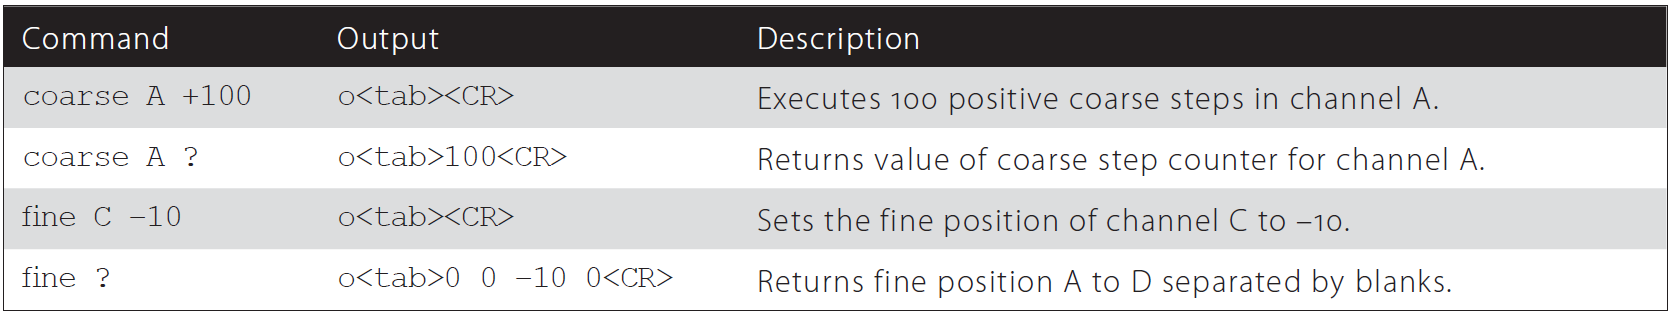
\includegraphics[width=\linewidth]{img/nc_func.png}
    \captionsource{Befehle, um die Position der Manipulatoren im Grob- und Feinbereich auszulesen und zu ändern. Auszug dem Nanocontrol Software Manual.}{Kleindiek Nanotechnik GmbH}
    \label{fig:nc_func}
\end{figure}
\newpage
Um die Bedienung des Manipulators zu vereinfachen und zu standardisieren, wird eine dedizierte Klasse in Python erstellt, die das Nanocontrol repräsentiert. Die Implementierung dieser Klasse kann Abbildung \ref{fig:ncumldiag} entnommen werden. Innerhalb dieser Klasse sind alle für den Manipulator verfügbaren Befehle in Python-Funktionen eingebettet. Diese Funktionen sind mit entsprechenden Tests versehen, um die korrekte Eingabe zu gewährleisten. Dies stellt eine einfache und sichere Bedienung des Manipulators über den Python-Code sicher und trägt zur Robustheit des Gesamtsystems bei.

Die Controller-Klasse – ebenfalls in Abbildung \ref{fig:ncumldiag} dargestellt ist – ist für die Erzeugung von Instanzen aller angeschlossenen Nanocontrols verantwortlich. Zur Erzeugung des Datensatzes werden acht Manipulatoren und ein Tisch verwendet. Die automatisierte Ansteuerung wird ebenfalls über den Controller realisiert.

Die Implementierung der Schnittstelle des Nanocontrols in Python bietet eine flexible und anpassbare Lösung zur Steuerung der Manipulatoren durch speziell entwickelte Skripte. Dies ist besonders nützlich, um systematisch eine Vielzahl von Szenarien und Bedingungen für die Erstellung des Datensatzes abzudecken.
\begin{figure}[h]
    \centering
\begin{tikzpicture}[scale=1]
  \umlclass[x=8,y=-1, scale=0.8]{COMDevice}{
    - port : str \\
    - baudrate : int \\
    - ser : Serial
  }{
    + \_\_init\_\_(port: str, baudrate: int) \\
    + open() : void \\
    + close() : void \\
    + send(data: str) : void \\
    + receive() : str \\
    + isConnected() : bool
  }

  \umlclass[x=0,y=-4, scale=0.8]{NanoControl}{
    - port : str \\
    - ser : COMDevice
  }{
    + \_\_init\_\_(port: str) \\
    + close() : void \\
    + stop(ack: bool = True) : str \\
    + getVersion() : str \\
    + getInfo() : dict \\
    + getCoarseCounters(axis: Optional[str] = None) : dict \\
    + moveCoarse(axis: str, steps: int, speed: Optional[int] = None) : str \\
    + resetCoarseCounter(axis: Optional[str] = None) : str \\
    + getFinePos12Bit(axis: Optional[str] = None) : dict \\
    + getFinePos16Bit(axis: Optional[str] = None) : dict \\
    + getFinePosVoltage(axis: Optional[str] = None) : dict \\
    + setFinePos12Bit(axis: str, position: int) : str \\
    + setFinePos16Bit(axis: str, position: int) : str \\
    + setFinePosVoltage(axis: str, position: int) : str \\
    + moveFine12Bit(axis: str, steps: int) : str \\
    + moveFine16Bit(axis: str, steps: int) : str \\
    + setSpeed(s: int) : str \\
    + getSpeed() : dict \\
    + setSpeedConfig(movement: Dict[str, Tuple[str, int]], speed: int) : str \\
    + turnKnobs(a: int, b: int, c: int, d: int) : str \\
    + moveAxesFWC(a: int, b: int, c: int, d: int) : str \\
    + moveAxisContinuousFWC(a: int, b: int, c: int, d: int, ms: int) : str \\
  }

  \umlclass[x=8,y=-7, scale=0.8]{Controller}{
    - ncs : dict \\
    - stage : dict \\
    - ncs\_pattern : dict \\
    - step : int \\
    - stagestep : int \\
    - patterns : dict \\
    - stage_pattern = []

    }{
    + \_\_init\_\_() \\
    + closeAll() \\
    + assignPattern(blocked\_tips: Any) \\
    + retractStep(factor: int = 1) \\
    + moveStage() \\
  }

  \umluniassoc{NanoControl}{COMDevice}

%  \umlinherit[geometry=|-|]{API\_ERROR\_Wrapper}{API\_ERROR}
%  \umlinherit[geometry=|-|]{SEM\_API\_CUSTOM}{API\_ERROR\_Wrapper}
  \umluniassoc{Controller}{NanoControl}
\end{tikzpicture}
    \caption{Die Implementierung der Schnittstelle des Nanocontrols in Python ermöglicht eine flexible Steuerung der Manipulatoren.}
    \label{fig:ncumldiag}
\end{figure}
\newpage
\section{Implementierung der GeminiSEM API in Python}
ZEISS stellt Entwicklern eine API zur Verfügung, um das REM in eigenentwickelten Programmen zu steuern. Zur Verwendung der bereitgestellten ocx-Datei, die unter Windows ein ActiveX-Steuerelement bereitstellt, wird die Python-Bibliothek pywin32 verwendet.
Die Nutzung der API in Python wird von ZEISS beispielhaft in dem GeminiSEM API Handbuch dargestellt und wird für die Implementierung die Klasse \glqq Sem\grqq{} genutzt. Sie bietet Funktionen zum Setzen und Auslesen der Parameter, die im Rahmen dieser Arbeit angepasst werden müssen, und enthält Funktionen wie \glqq grabFullImage(...)\grqq{}, \glqq grabMask()\grqq{} und \glqq grabImageWithParameters(...)\grqq{}, die für eine effiziente Bildaufnahme zur Erstellung des Datensatzes mit verschiedenen REM-Parametern entwickelt wurden. In Kapitel \ref{sec:bildaugpar} wird näher auf die in dieser Arbeit verwendeten Parameter eingegangen.
Es ist stets darauf zu achten, dass das REM ein vollständiges Bild aufnimmt. Dies wird sichergestellt, indem die Aufnahmedauer mit der Funktion getFrameTimeInSeconds() ausgelesen und berechnet wird.
Eine weitere wichtige Funktion ist das Rücksetzen des REM in den Ausgangszustand. Dies ist wichtig, da einige Parameter gleichzeitig geändert werden und ein späteres manuelles Zurücksetzen viel Zeit in Anspruch nehmen würde. Das korrekte Rücksetzen des REM wird durch die Funktionen \glqq getInitialParameters()\grqq{} und \glqq restoreInitialParameters()\grqq{} sichergestellt.

\begin{figure}[h]
    \centering
\begin{tikzpicture}[scale=1]
%  \umlclass[x=0,y=0]{API\_ERROR}{}{
%    + \_\_init\_\_(error\_code: int) \\
%  }
%
%  \umlclass[x=7,y=0]{API\_ERROR\_Wrapper}{}{
%    + \_\_error\_handling(func: Callable) \\
%  }
  \begin{umlpackage}[x=-4,y=0]{ActiveX Control}
    \umlclass[scale=0.7]{SemAPI}{}{
      + InitialiseRemoting() \\
      + GetVersion() \\
      + ClosingControl() \\
      + GetValue(AP\_name: str, style: str) \\
      + GetValueMin(AP\_name: str) \\
      + GetValueMax(AP\_name: str) \\
      + SetValue(AP\_name: str, value) \\
      + GetState(DP\_name: str, style: str) \\
      + SetState(DP\_name: str, value) \\
      + Execute(CMD\_name: str) \\
      + GetStagePosition() \\
      + MoveStage(coord) \\
      + Grab(fname: str, X: int, Y: int, W: int, H: int, overlay: bool) \\
      + GetCurrentUserName() \\
      + SetNotify(PARAM: str, value: bool)
    }
%    \umlnote[x=7, y=-5]{SEM\_API}{
%      Functions derived from SEM API and \\
%      interface for real-time image
%    }
  \end{umlpackage}
  \umlclass[x=4,y=0, scale=0.7]{Sem}{
    - ocx : SemAPI \\
    - initial\_parameters : Tuple \\
    - busy : bool \\
  }{
    - \_\_init\_\_() \\
    + openConnection() \\
    + closeConnection() \\
    + getInitialParameters() \\
    + restoreInitialParameters() \\
    + grabFullImage(fname: str, overlay: bool) \\
    + grabImageWithParameters(dest: str, mag: str, rot: str,\\ \hspace{2cm}detector: str, scanrate: str, wd: float) \\
    + grabMask() \\
    + getAPMag() \\
    + setAPMag(mag: str \\
    + getAPWD() \\
    + setAPWD(wd: float) \\
    + getAPRot() \\
    + setAPRot(rot: str) \\
    + getDPDetector() \\
    + setDPDetector(detector: str) \\
    + getDPScanrate() \\
    + setDPScanrate(scanrate: str) \\
    + getAPFrameTimeInSeconds() \\
  }

  \umluniassoc{Sem}{SemAPI}
\end{tikzpicture}
    \caption{Die SemAPI wird von ZEISS in Form einer ocx-Datei zur Verfügung gestellt. Die Sem-Klasse bietet eine abstrahierte und angepasste Form der API, die speziell für die effiziente Erstellung von Datensätzen geeignet ist.}
    \label{fig:semumldiag}
\end{figure}

\section{Aufnahme der Bilddaten}
Die spezifischen Methoden und Techniken, die zur automatisierten Erfassung der Bilder für den Datensatz entwickelt wurden, werden im folgenden Abschnitt detailliert beschrieben.

Der für dieses Projekt entwickelte Datensatz besteht aus zwei Teilen. Der erste Teil umfasst 150 Bilder aus realen Einsätzen, die bereits vorhanden sind und lediglich annotiert werden müssen. Diese Bilder bestehen hauptsächlich aus Aufnahmen, bei denen die Spitzen eine Probe kontaktieren. Dies ist die Zielposition der Spitzen und erfordert die höchste Genauigkeit, weshalb hier auf eine Bildaugmentation verzichtet wird und nur Aufnahmen aus realen Szenarien verwendet werden.
Der zweite Teil besteht aus 600 Bildern und 100 zugehörigen Masken, die für die Erstellung des Datensatzes aufgenommen wurden.
Der Begriff \glqq Masken\grqq{} bezieht sich in diesem Zusammenhang auf Bilder, die später speziell eingefärbt werden, um die genaue Position und Form der Nadeln in den Datensätzen zu markieren. Auf diese Weise wird eine direkte Beziehung zwischen den Bildern und den Positionen der Nadeln hergestellt, was für das Training des Modells von entscheidender Bedeutung ist. Die Masken dienen während des Trainingsprozesses als \glqq Wahrheitsquelle\grqq{} und ermöglichen es dem Modell zu lernen, wie Nadeln in den Bildern erkannt und lokalisiert werden können.

Zur Erzeugung der Bilder wird eine Art Bildaugmentation entwickelt. Dabei werden die Parameter des Mikroskops genutzt, um Rauschen und Unschärfe einzubringen und die Lichtverhältnisse zu variieren. Durch Veränderung der Probenposition wird der Hintergrund variiert. So kann ein und dieselbe Szene auf unterschiedliche Weise aufgenommen werden. Die Erstellung eines umfassenden Datensatzes wird dadurch beschleunigt.
Für die Aufnahme der Masken sind die Parameter so gewählt, dass die Bilder einen starken Kontrast, scharfe Kanten und ein hohes Signal-Rausch-Verhältnis aufweisen. Dies erleichtert die spätere Annotation, da die Konturen der Spitzen leicht und akkurat identifiziert werden können.

\subsection{Variation der aufzunehmenden Szene}
Die Anordnung der Spitzen im Sichtfeld des REM und die Vielfalt der Szenen, die sie erzeugen, spielen eine zentrale Rolle bei der Erstellung des Datensatzes. 
Zunächst ist zu beachten, dass in der Regel acht Nadeln auf dem Prober Shuttle montiert sind, aber nur ein Teil davon tatsächlich im Sichtfeld des REM liegt. Die Nadeln können sich kreuzen und Teile einer Nadel verdecken, oder es kann nur ein sehr kleiner Teil in das Bild ragen, was die Erkennung erschwert.

Der Vergrößerungsfaktor hat, wie in Abbildung \ref{fig:mags} zu sehen ist, ebenfalls einen großen Einfluss auf die Darstellung der Spitzen.
\begin{figure}[htbp]
    \centering
    \subfigure[30000-fache Vergrößerung]{\label{subfig:30kmag}
    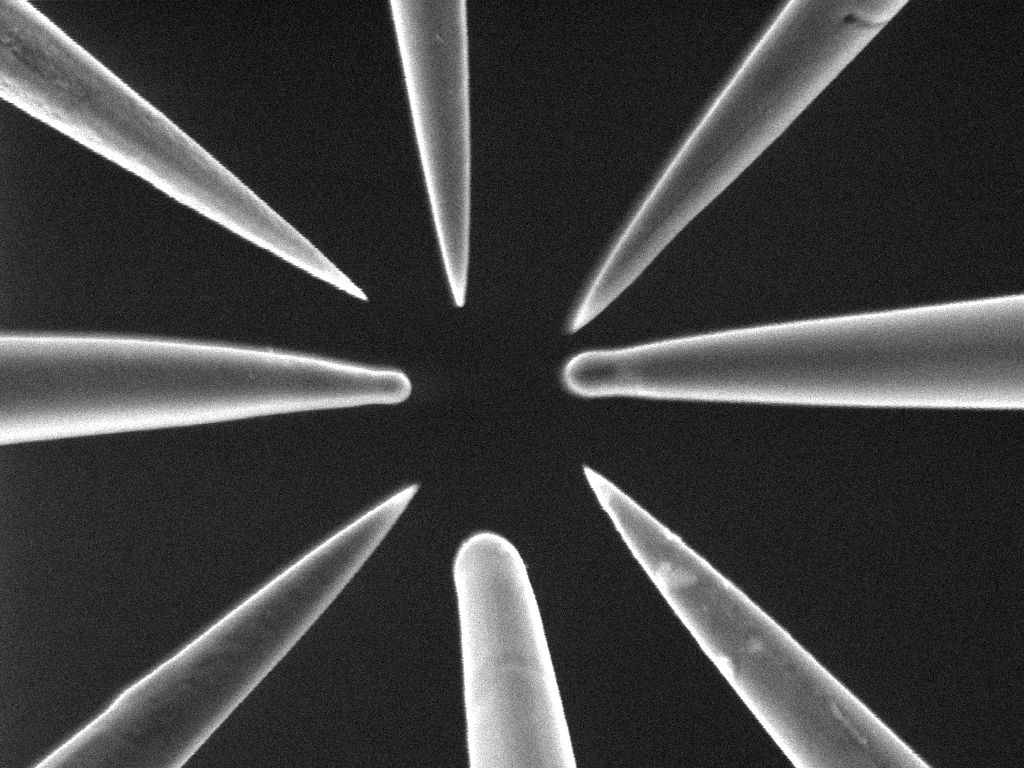
\includegraphics[width=0.32\textwidth]{img/30000x_image005.png}}
    \subfigure[10000-fache Vergrößerung]{\label{subfig:10kmag}
    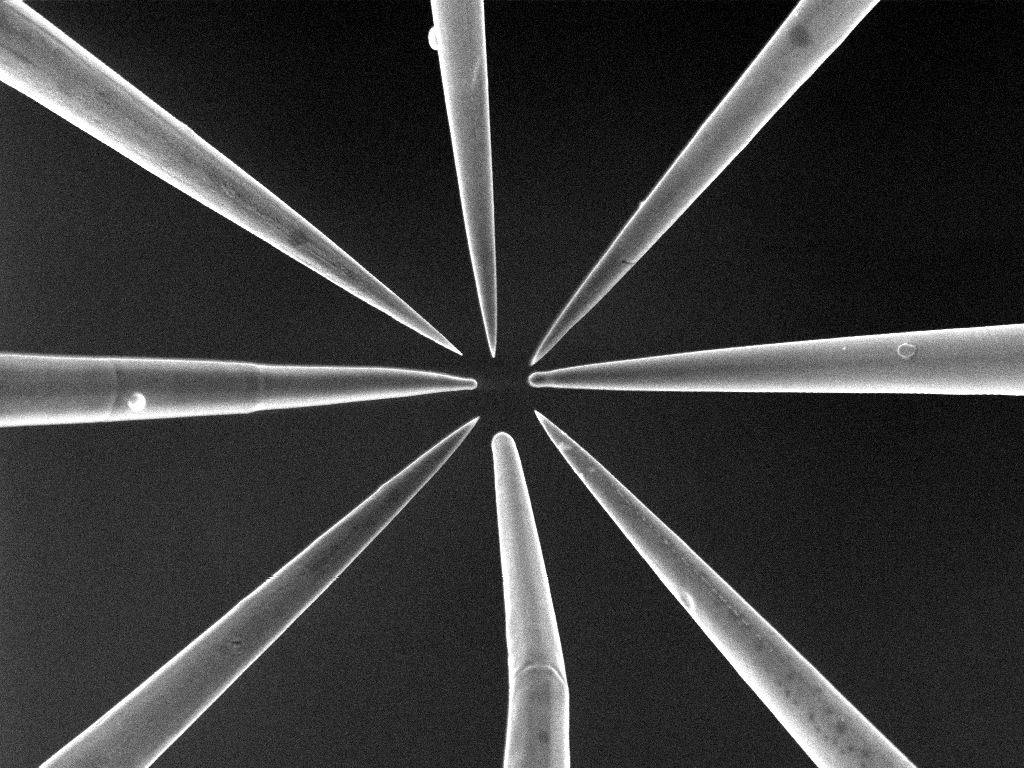
\includegraphics[width=0.32\textwidth]{img/10000x_image007.png}}
    \subfigure[2000-fache Vergrößerung]{\label{subfig:2kmag}
    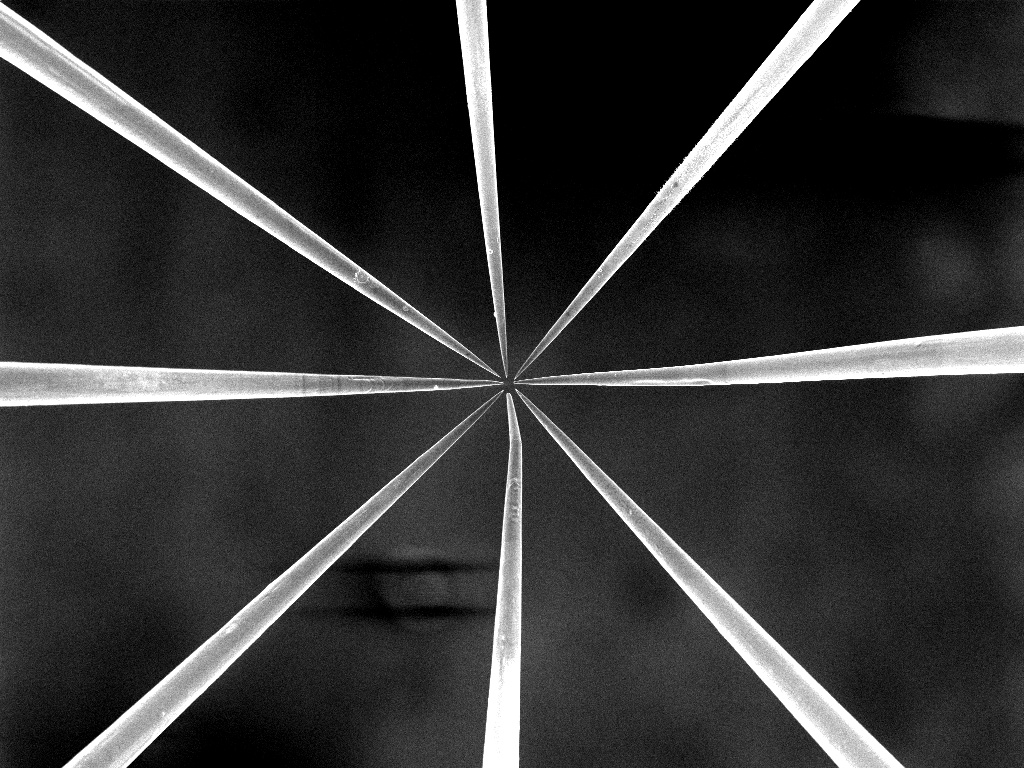
\includegraphics[width=0.32\textwidth]{img/2000x_image009.png}}
    \caption{Messspitzen, dargestellt bei unterschiedlichen Vergrößerungen. Bei einer hohen Vergrößerung sind die Spitzen klar erkennbar. Je kleiner die Vergrößerung, desto schwerer ist es, den Apex der Spitze zu lokalisieren.}
    \label{fig:mags}
\end{figure}
Durch die Aufnahme von Bildern bei verschiedenen Vergrößerungen, wird sichergestellt, dass das trainierte Modell später in der Lage ist, die Messspitzen unabhängig vom Vergrößerungsfaktor zu erkennen und zu lokalisieren.

Ein weiterer wichtiger Aspekt ist die Untergrundvariation. Hierbei handelt es sich um die strategische Verschiebung der Probe im REM. Je nach Position und Ausrichtung der Probe können unterschiedliche Strukturen wie SRAM-Zellen, Metallisierungsebenen, Transistoren oder andere mikro- und nanoskalige Strukturen, die typischerweise in einem Halbleiterchip vorkommen, im Hintergrund erscheinen und das Gesamtbild erheblich beeinflussen. Durch diese Variation des Hintergrunds wird das trainierte Modell widerstandsfähiger gegen Hintergrundstrukturen, die den Nadeln ähnlich sehen. Dies ist ein wichtiger Schritt, um sicherzustellen, dass das später trainierte Modell eine niedrige FP-Rate aufweist.
Schließlich ist es wichtig, dass eine Vielzahl von Positionen, an denen sich die Spitzen befinden, im Datensatz vertreten sind. Dies wird durch das Anfahren verschiedener Positionen mit den Spitzen erreicht. 

Durch Berücksichtigung der genannten Faktoren, wird sichergestellt, dass der Datensatz eine große Vielfalt realer Bedingungen widerspiegelt, unter denen das Modell funktionieren soll.

\subsection{Bildaugmentierung durch REM-Parameter}
\label{sec:bildaugpar}
Die Augmentierung der Trainingsdaten spielt eine wichtige Rolle beim maschinellen Lernen und wird verwendet, um die Menge der Trainingsdaten zu erhöhen und das Modell robuster gegenüber Änderungen der Eingangsdaten zu machen. Üblicherweise werden in der Bildverarbeitung Techniken wie Drehen, Beschneiden, Verzerren oder Verrauschung verwendet. In dieser Arbeit wird jedoch ein alternativer Ansatz zur Augmentierung gewählt.
Die Augmentierung der Bilder durch Variation der REM-Parameter anstelle einer Nachbearbeitung der Bilder hat mehrere Vorteile.

Erstens ermöglicht diese Methode ein realistischeres Verrauschen der Bilder. Das Rauschen in REM-Bildern hat eine besondere Charakteristik, die durch nachträgliche Rauschaddition nicht einfach reproduziert werden kann.
Zweitens spielt die Variation der Unschärfe eine wichtige Rolle. Da die Spitzen sich meist auf unterschiedlichen Höhen befinden, wirkt sich die Unschärfe nicht gleichmäßig auf das gesamte Bild aus. Bei einer nachträglichen Bearbeitung würde das gesamte Bild unscharf erscheinen, was nicht der Realität entspricht.
Drittens hat die Variation des Kontrasts durch unterschiedliche Sekundärelektronendetektoren einen erheblichen Einfluss auf das Bild. Eine einfache Kontraständerung in der Nachbearbeitung würde diese Effekte nicht berücksichtigen.

Zusammenfassend lässt sich sagen, dass die Variation der REM-Parameter während der Bildaufnahme eine realistischere und anwendungsspezifische Augmentierung ermöglicht, die den Anforderungen besser entspricht. Im Folgenden werden die einzelnen Parameter und ihre Auswirkungen näher erläutert.

Zunächst spielt die Vergrößerung eine zentrale Rolle. Sie bestimmt den beobachteten Bereich und beeinflusst somit die Darstellung der Spitzen und der Probe. Wie in Abbildung \ref{fig:mags} zu sehen ist, sind die Spitzen bei niedriger Vergrößerung fast über ihre gesamte Länge sichtbar, sie erscheinen sehr dünn und lang, und der vordere Punkt der Spitze ist schwer zu lokalisieren. Bei hoher Vergrößerung hingegen nehmen die Spitzen einen großen Teil des Bildes ein und die feinen Strukturen der Probe, wie zum Beispiel einzelne Transistoren, werden sichtbar. Aus diesem Grund werden für die Erstellung des Datensatzes verschiedene Vergrößerungsstufen verwendet, nämlich 50000-, 25000-, 10000- und 2000-fache Vergrößerung.

\begin{table}[h]
\begin{center}
\begin{tabular}{lll}
\toprule
Bezeichnung&Beschreibung&Einheit\\
\midrule
AP\_MAG&Vergrößerung&-\\
AP\_WD&Arbeitsdistanz&\SI{}{\metre}\\
AP\_SCANROTATION&Rotation der Abtastrichtung&\SI{}{\degree}\\
AP\_FRAME\_TIME&Zykluszeit eines Bildes&\SI{}{\milli\second}\\
\bottomrule
\end{tabular}
\end{center}
\caption{Auszug aus den genutzten analogen Parametern des ZEISS GeminiSEM.}
\label{tab:AP_Parameter}
\begin{small}
\end{small}
\end{table}
Ein weiterer wichtiger Parameter ist die Arbeitsdistanz. Sie beeinflusst die Bildschärfe und stellt oft eine Herausforderung bei der richtigen Einstellung dar. Um eine Variation in der Bildschärfe zu erzeugen und damit das Modell auf unterschiedliche Schärfegrade zu trainieren, werden Bilder entweder bei exakt eingestelltem Arbeitsabstand – wenn die Spitzen im Fokus sind – oder bei einem um 0,5 Prozent reduzierten Arbeitsabstand aufgenommen. Dadurch soll das mit den Daten trainierte Modell später in der Lage sein, auch unscharfe Spitzen korrekt zu lokalisieren.
\newpage
Um sicherzustellen, dass der Datensatz auch stark verrauschte Bilder enthält, werden verschiedene Abtastraten verwendet. Die Abtastrate des REM bestimmt, wie schnell die Szene mit dem Elektronenstrahl abgetastet wird. Dies beeinflusst das Signal-Rausch-Verhältnis des Bildes. Eine niedrige Abtastrate führt zu einem geringeren Signal-Rausch-Verhältnis, liefert aber bis zu 5 Bilder pro Sekunde, während bei höheren Abtastraten die Aufnahme eines Bildes bis zu mehreren Minuten dauern kann, dafür aber von besserer Qualität ist. Die Bilder für den Datensatz werden mit den Abtastraten 2 und 6 aufgenommen. Diese entsprechen den in der Praxis am häufigsten verwendeten Abtastraten bei Kleindiek Nanotechnik. Dadurch werden sowohl verrauschte als auch gut aufgelöste Bilder erzeugt.

Schließlich haben die verwendeten Detektoren des REM, InLens und SE2 einen großen Einfluss auf die Helligkeit und den Kontrast der Bilder. Die Verwendung unterschiedlicher Detektoren ermöglicht die Aufnahme von Bildern unter verschiedenen Beleuchtungs- und Kontrastbedingungen.
Zur Erstellung der Masken wird der SE2 Detektor genutzt. Bei einer langsamen Abtastrate von 10, welche ungefähr einem Bild pro Minute entspricht, liefert dieser Bilder, auf denen die Konturen der Nadeln deutlich erkennbar sind.

Eine Rotation der Abtastrichtung wurde anfangs in Betracht gezogen, wurde aber nach einigen Tests wieder verworfen, da die Änderung der anderen Parameter bereits ausreicht, um eine Szene ausreichend abzubilden. Es wurde festgestellt, dass eine Rotation der Bilder durch das REM keinen zusätzlichen Nutzen bringt. Sie würde lediglich dazu führen, dass zu viele Bilder der gleichen Szene im Datensatz enthalten sind. Außerdem kann eine Rotation nachträglich auf die Bilder angewendet werden, wenn dies gewünscht wird. 
\begin{table}[h]
\begin{center}
\begin{tabular}{llll}
\toprule
Bezeichnung&Beschreibung&Wert&Text\\
\midrule
DP\_SCAN\_ROT&Rotation der Abtastung&0&Aus\\
&&1&An\\
DP\_FREEZE\_ON&Abtastung einfrieren&0&Ende des Bildes\\
&&1&Ende der Zeile\\
&&2&Nach Befehl\\
DP\_SCANRATE&Abtastungsrate&0-21&0-21\\
DP\_FROZEN&Abtastung&0&Live\\
&&1&Eingefroren\\
DP\_DETECTOR\_TYPE&Aktiver Detektor&0-37&2=SE2, 9=InLens\\
\bottomrule
\end{tabular}
\end{center}
\caption{Auszug aus den genutzten digitalen Parametern des ZEISS GeminiSEM.}
\label{tab:DP_Parameter}
\begin{small}
\end{small}
\end{table}
\newpage
\subsection{Automatisierung}
Bei der automatisierten Aufnahme wird der Abtastvorgang in umgekehrter Reihenfolge durchgeführt. Das bedeutet, dass die Nadeln von ihrer Endposition, die einem Radius von \SI{1}{\micro\metre} entspricht, bis zu einem Radius von \SI{50}{\micro\metre} zurückgezogen werden. Um Beschädigungen zu vermeiden, muss sichergestellt werden, dass sich die Spitzen während des Rückzugs nicht gegenseitig berühren. Dies wird durch die Verwendung vordefinierter Bahnen erreicht. Bei acht montierten Spitzen ergibt sich ein Bereich von 45 Grad, in dem die Spitzen ohne Kollisionsgefahr zurückgezogen werden können. Die für diesen Prozess verwendeten spezifischen Pfade sind in Abbildung \ref{fig:pathmanip} dargestellt.

Nach manueller Positionierung der Spitzen in der Startposition für die Aufnahme (Radius von \SI{1}{\micro\metre}) und Einstellung beider Detektoren auf ein scharfes Bild startet die speziell entwickelte Routine. Dargestellt als Pseudocode wird diese Routine in Algorithmus \ref{alg:Pseudocode}.
\begin{figure}[htbp]
  \centering
  \subfigure[Tip]{
  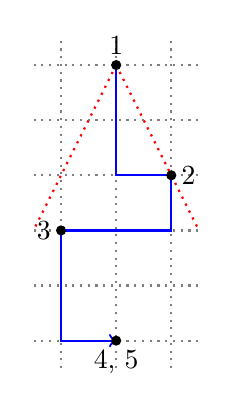
\begin{tikzpicture}[thick, scale=0.7]
      \draw[dotted, gray] (-1.5,-5.5) grid (1.5,0.5); % Dotted grid
      \draw[dotted, red] (0,0) -- (1.5,-3);
      \draw[dotted, red] (0,0) -- (-1.5,-3);
      \draw[blue,->] (0,0) -- (0,-2) -- (1,-2) -- (1,-3) -- (-1,-3) -- (-1,-5) -- (0,-5);
      \filldraw[black, thick] (0,0) circle (2pt) node[above] {1};
      \filldraw[black, thick] (1,-2) circle (2pt) node[right] {2};
      \filldraw[black, thick] (-1,-3) circle (2pt) node[left] {3};
      \filldraw[black, thick] (0,-5) circle (2pt) node[below] {4, 5};
  \end{tikzpicture}}
  \subfigure[Tip]{
  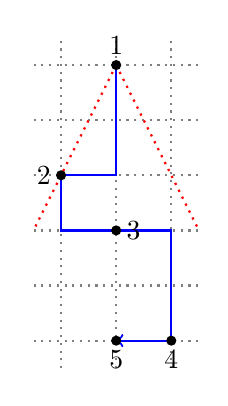
\begin{tikzpicture}[thick,scale=0.7]
      \draw[dotted, gray] (-1.5,-5.5) grid (1.5,0.5); % Dotted grid
      \draw[blue,->] (0,0) -- (0,-2) -- (-1,-2) -- (-1,-3) -- (0,-3) -- (1,-3) -- (1,-5) -- (0,-5);
      \draw[dotted, red] (0,0) -- (1.5,-3);
      \draw[dotted, red] (0,0) -- (-1.5,-3);
      \filldraw[black, thick] (0,0) circle (2pt) node[above] {1};
      \filldraw[black, thick] (-1,-2) circle (2pt) node[left] {2};
      \filldraw[black, thick] (0,-3) circle (2pt) node[right] {3};
      \filldraw[black, thick] (1,-5) circle (2pt) node[below] {4};
      \filldraw[black, thick] (0,-5) circle (2pt) node[below] {5};
  \end{tikzpicture}}
  \subfigure[Tip]{
  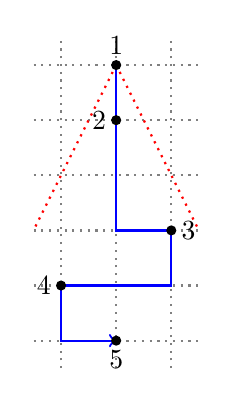
\begin{tikzpicture}[thick, scale=0.7]
      \draw[dotted, gray] (-1.5,-5.5) grid (1.5,0.5); % Dotted grid
      \draw[blue,->] (0,0) -- (0,-3) -- (1,-3) -- (1,-4) -- (-1,-4) -- (-1,-5) -- (0,-5);
      \draw[dotted, red] (0,0) -- (1.5,-3);
      \draw[dotted, red] (0,0) -- (-1.5,-3);
      \filldraw[black, thick] (0,0) circle (2pt) node[above] {1};
      \filldraw[black, thick] (0,-1) circle (2pt) node[left] {2};
      \filldraw[black, thick] (1,-3) circle (2pt) node[right] {3};
      \filldraw[black, thick] (-1,-4) circle (2pt) node[left] {4};
      \filldraw[black, thick] (-0,-5) circle (2pt) node[below] {5};
  \end{tikzpicture}}
  \subfigure[Tip]{
  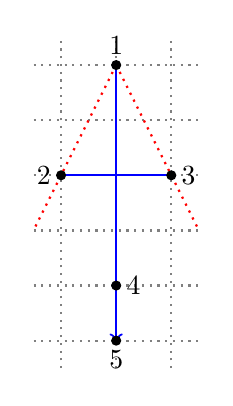
\begin{tikzpicture}[thick, scale=0.7]
      \draw[dotted, gray] (-1.5,-5.5) grid (1.5,0.5); % Dotted grid
      \draw[blue,->] (0,0) -- (0,-2) -- (-1,-2) -- (1,-2) -- (0,-2) -- (0,-4) -- (0,-5);
      \draw[dotted, red] (0,0) -- (1.5,-3);
      \draw[dotted, red] (0,0) -- (-1.5,-3);
      \filldraw[black, thick] (0,0) circle (2pt) node[above] {1};
      \filldraw[black, thick] (-1,-2) circle (2pt) node[left] {2};
      \filldraw[black, thick] (1,-2) circle (2pt) node[right] {3};
      \filldraw[black, thick] (0,-4) circle (2pt) node[right] {4};
      \filldraw[black, thick] (0,-5) circle (2pt) node[below] {5};
  \end{tikzpicture}}
  \subfigure[Stage]{
  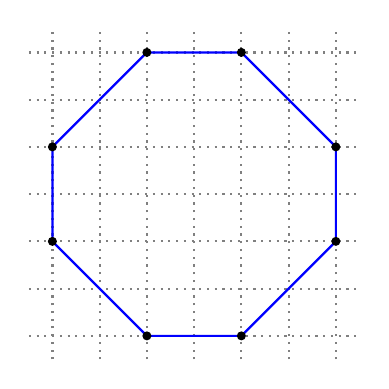
\begin{tikzpicture}[thick, scale=0.6]
      \draw[dotted, gray] (-2.5,-0.5) grid (4.5,6.5); % Dotted grid
      \draw[blue,-] (0,0) -- (2,0) -- (4,2) -- (4,4) -- (2,6) -- (0,6) -- (-2,4) -- (-2,2) -- (0,0);
      \filldraw[black] (0,0) circle (2pt);
      \filldraw[black] (2,0) circle (2pt);
      \filldraw[black] (4,2) circle (2pt);
      \filldraw[black] (4,4) circle (2pt);
      \filldraw[black] (2,6) circle (2pt);
      \filldraw[black] (0,6) circle (2pt);
      \filldraw[black] (-2,4) circle (2pt);
      \filldraw[black] (-2,2) circle (2pt);
  \end{tikzpicture}}
  \caption{Vier vordefinierte Pfade für das Zurückziehen der Messspitzen. Der Verfahrweg wird mit der Vergrößerung skaliert. Die Probe wird zyklisch verfahren.}
  \label{fig:pathmanip}
\end{figure}

Zunächst wird jedem Manipulator ein zufälliger Pfad zugewiesen, den er abfahren wird. Anschließend wird eine Maske eingezogen, die später für die Annotation verwendet wird.
Das System nimmt nun eine vordefinierte Anzahl von Bildern der eingestellten Szene auf. Für jedes Bild wird eine zufällige Konstellation von REM-Parametern aus einem vordefinierten Satz ausgewählt. Die Probe wird zwischen jedem Bild an eine andere Position bewegt. Dazu ist eine zyklische Bahn definiert und die Probe wird so ausgerichtet, dass sie auf dem Pfad eine möglichst große Variation der Probenstruktur abdeckt. Da die Spitzen während der Aufnahme der fünf Bilder ihre Position beibehalten, kann die zuvor erstellte Maske zur Markierung der Spitzenposition für alle Bilder der Szene verwendet werden.

\begin{figure}[h]
    \centering
    \subfigure[]{
    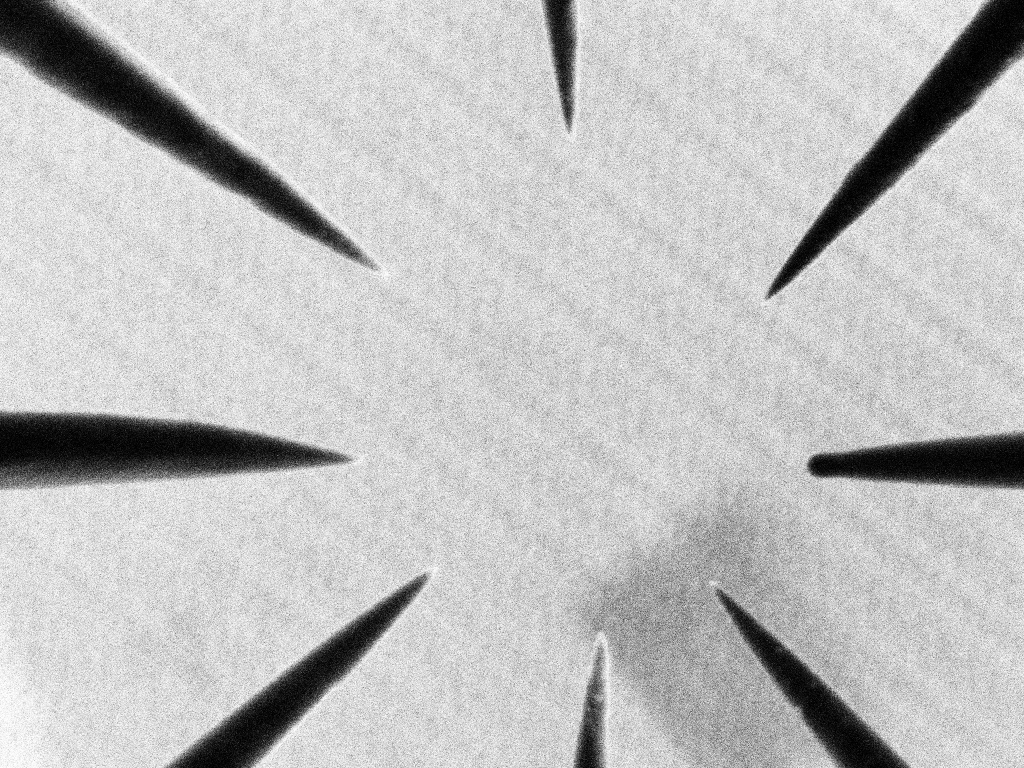
\includegraphics[width=.3\linewidth]{img/000.png}
    \label{fig:augimg0}
    }
    \subfigure[]{
    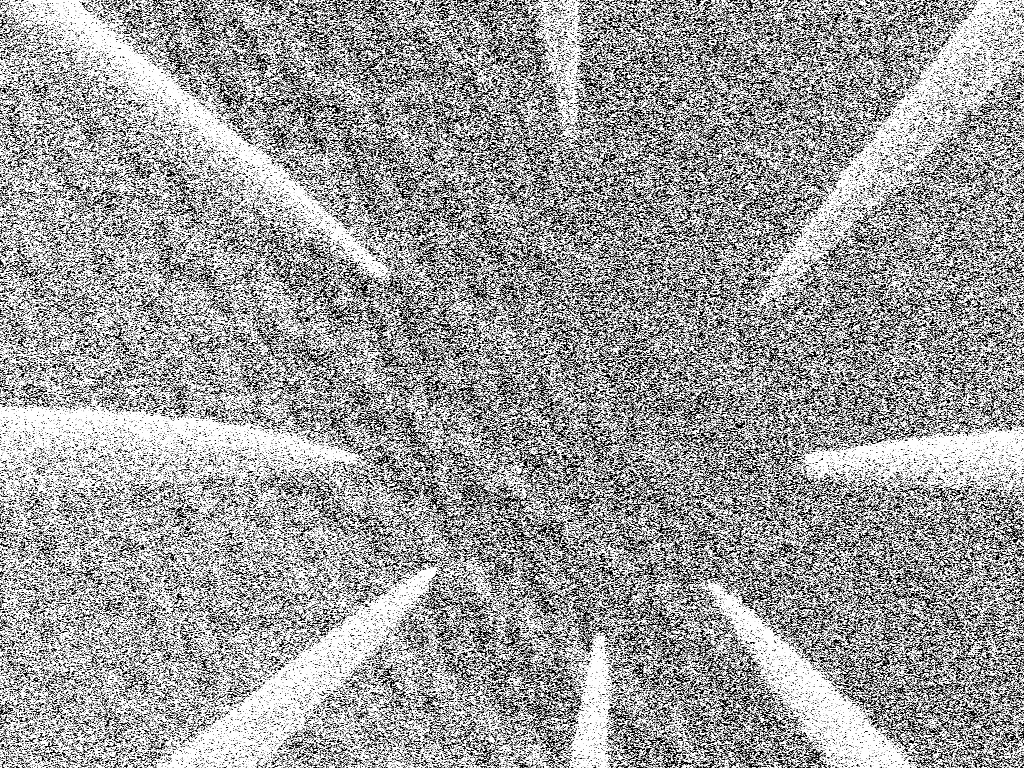
\includegraphics[width=.3\linewidth]{img/001.png}
    \label{fig:augimg1}
    }
    \subfigure[]{
    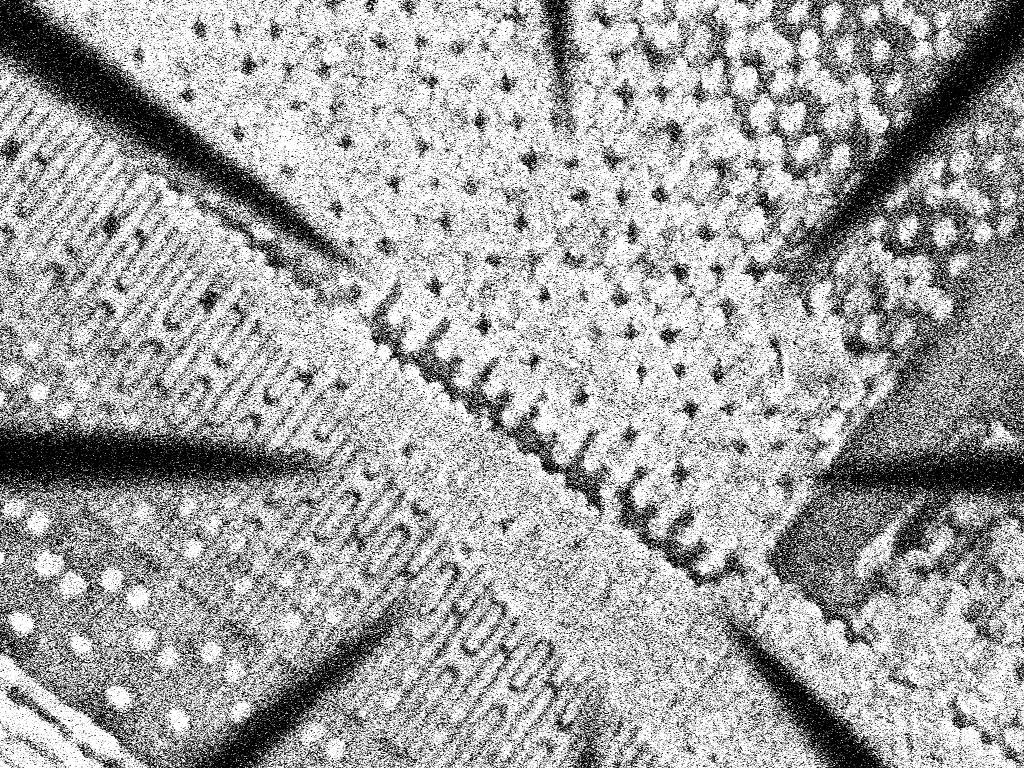
\includegraphics[width=.3\linewidth]{img/002.png}
    \label{fig:augimg2}
    }
    \subfigure[]{
    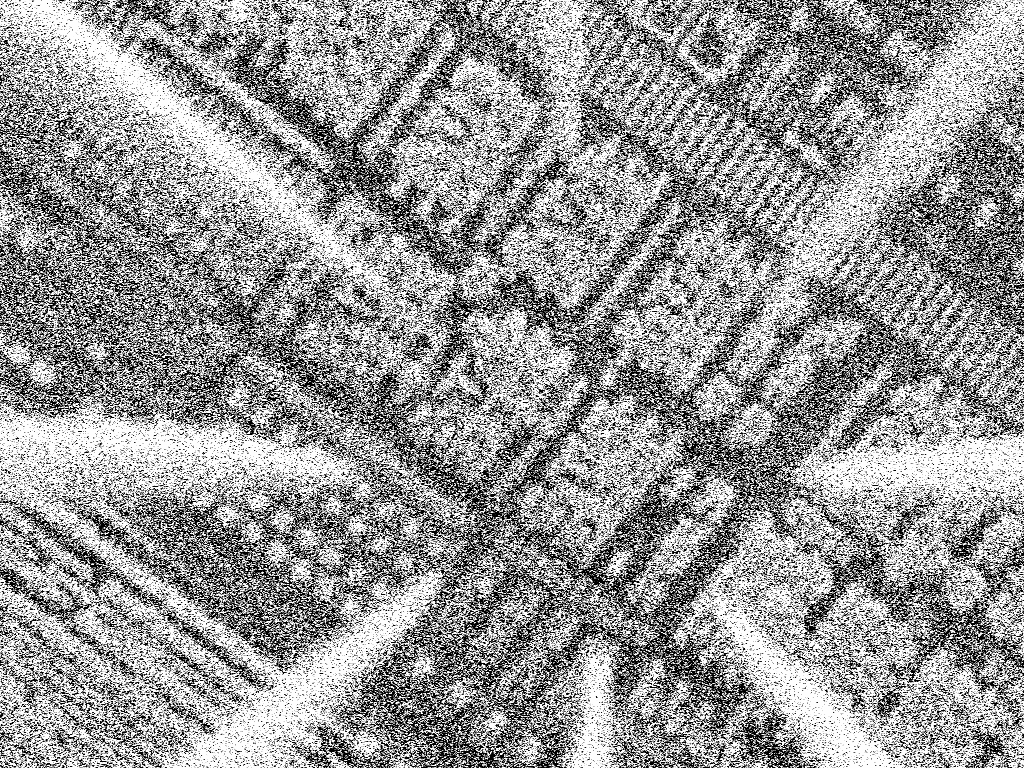
\includegraphics[width=.3\linewidth]{img/003.png}
    \label{fig:augimg3}
    }
    \subfigure[]{
    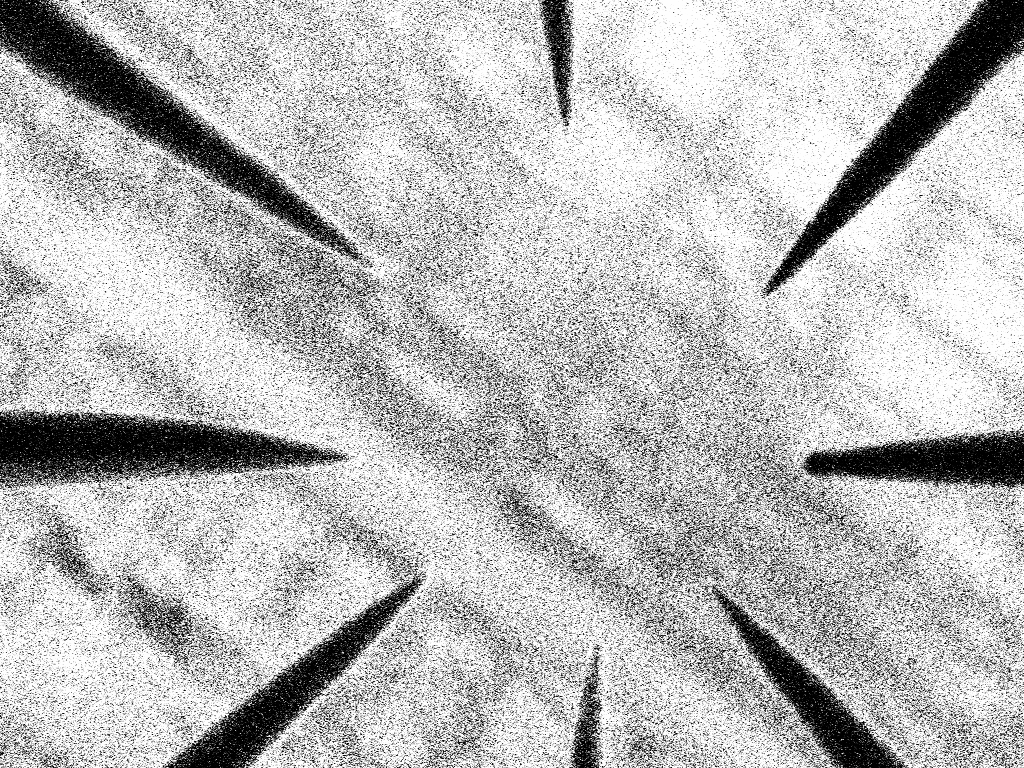
\includegraphics[width=.3\linewidth]{img/004.png}
    \label{fig:augimg4}
    }
    \caption{Eine Szene aufgenommen mit verschiedenen Parametern. Deutlich zu erkennen ist der Unterschied zwischen dem SE2 Detektor in (a), (c) und (e) und dem InLens Detektor in (b) und (d). Die Probenstruktur ist sehr unterschiedlich.}
    \label{fig:augimg}
\end{figure}
Dadurch reduziert sich der Aufwand für die nachfolgende Annotation auf ein Fünftel. Dieser Vorgang wird wiederholt, bis alle Spitzen die Endposition der ihnen zugewiesenen Pfade erreicht haben. Dann wird die nächst kleinere Vergrößerungsstufe (beginnend bei 50.000x, dann 25.000x, 10.000x und zuletzt 2.000x) verwendet und der Vorgang wiederholt.

Es ist wichtig, die zeitlichen Anforderungen dieses Prozesses zu berücksichtigen. Im Vorfeld wird viel Zeit darauf verwendet, die Nadeln in ihre Ausgangsposition zu bringen und die Parameter für ein scharfes Bild einzustellen. Beide Prozesse erfordern eine Reihe fein abgestimmter Einstellungen, die alle miteinander interagieren. Außerdem dauert ein einzelner Durchlauf der Routine etwa eine Stunde. Trotz dieser Herausforderungen stellt die automatisierte Bildaufnahme einen effizienten Ansatz dar, um eine große Anzahl von Bildern mit variablen Parametern zu erzeugen.

\begin{algorithm}[h!]
\begin{algorithmic}[1]
\caption{Routine für das automatische Einziehen der Bilder.}
\label{alg:Pseudocode}
\REQUIRE{Liste von Vergrößerungen: mags, Anzahl an Bildern pro Szene: count, Verwendete Abtastraten: srs, Verwendete Detektoren: dets, Zwei Arbeitsdistanzen: wds}
\ENSURE{Einen Datensatz an Bildern}
\FOR{mag \textbf{in} mags}
  \STATE controller.assignPattern()
  \COMMENT{Weise jedem Manipulator einen zufälligen Pfad zu}
  
  \FOR{$i \leftarrow 0$ \textbf{to} controller.patternLength()}
    \STATE sem.grabImage(mag, dt='SE2', sr='10', wds[0])
    \COMMENT{Ziehe ein Maskenbild ein.}
    \FOR{$j \leftarrow 0$ \textbf{to} count}
        \STATE wd, sr, dt $\leftarrow$ random(wds, srs, dts)
        \COMMENT{Wähle zufällige Mikroskop Parameter}
        \STATE sem.grabImage(mag, dt, sr, wd)
        \COMMENT{Ziehe ein Bild ein.}
        \STATE controller.moveStage()
        \COMMENT{Bewege die Probe.}
    \ENDFOR
    \STATE controller.restractStep()
    \COMMENT{Bewege die Manipulatoren}
  \ENDFOR
\ENDFOR
\end{algorithmic}
\end{algorithm}
\subsection{Ergebnis}
Bei einem Durchlauf der Routine, mit vier Vergrößerungsstufen, fünf Spitzenpositionen
und fünf Bildern pro Szene, werden insgesamt 100 Bilder und 20 Masken
erzeugt. Diese Routine wird sechsmal durchgeführt, jeweils mit verschiedenen
Ausgangspositionen der Spitzen und verschiedenen Positionen der Probe. Somit
ergeben sich insgesamt 600 Bilder und 100 zugehörige Masken.
\clearpage
\section{Daten Annotation}
\subsection{Segmentierung}
Bei der Erstellung der Annotation der Masken, wird bewusst auf polygonbasierte Werkzeuge verzichtet, da diese eine pixelgenaue Segmentierung erschweren. Daher wird Adobe Photoshop \cite{adobephotoshop} als Werkzeug der Wahl eingesetzt. Photoshop bietet eine Reihe von Werkzeugen, wie das \glqq Magnetic Lasso\grqq{} und \glqq Quick Select\grqq{}, die eine pixelgenaue Auswahl von Objekten erleichtern.

Um die Annotation zu vereinfachen und zu standardisieren, werden acht optisch und numerisch deutlich unterscheidbare Farben zur Markierung der Spitzen verwendet. Dabei wird darauf geachtet, dass den Spitzen aus einer bestimmten Himmelsrichtung immer die gleiche Farbe zugewiesen wird. Dies ermöglicht nicht nur die Unterscheidung der Instanzen, sondern gibt unter Berücksichtigung der Bildrotation auch Auskunft darüber, in welchem Manipulator die Spitze montiert ist. Nachdem alle Spitzen markiert sind, wird der restliche Bildbereich schwarz eingefärbt.

Um die Qualität der Annotationen sicherzustellen, wird mit Experten von Kleindiek definiert, welche Bereiche zu den Spitzen gehören und wie die Konturen zu zeichnen sind.

\begin{figure}[htbp]
    \centering
    \subfigure[Rohbild]{
    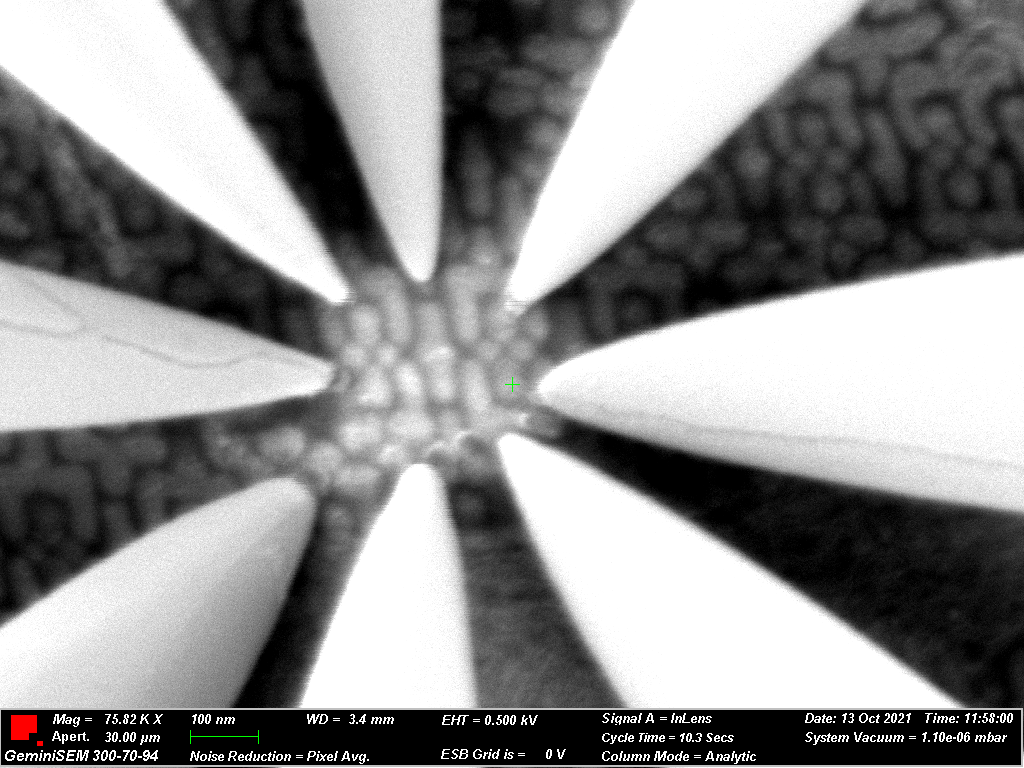
\includegraphics[width=0.45\linewidth]{img/drifttest_stop_017_0.png}
    }
    \subfigure[Maske]{
    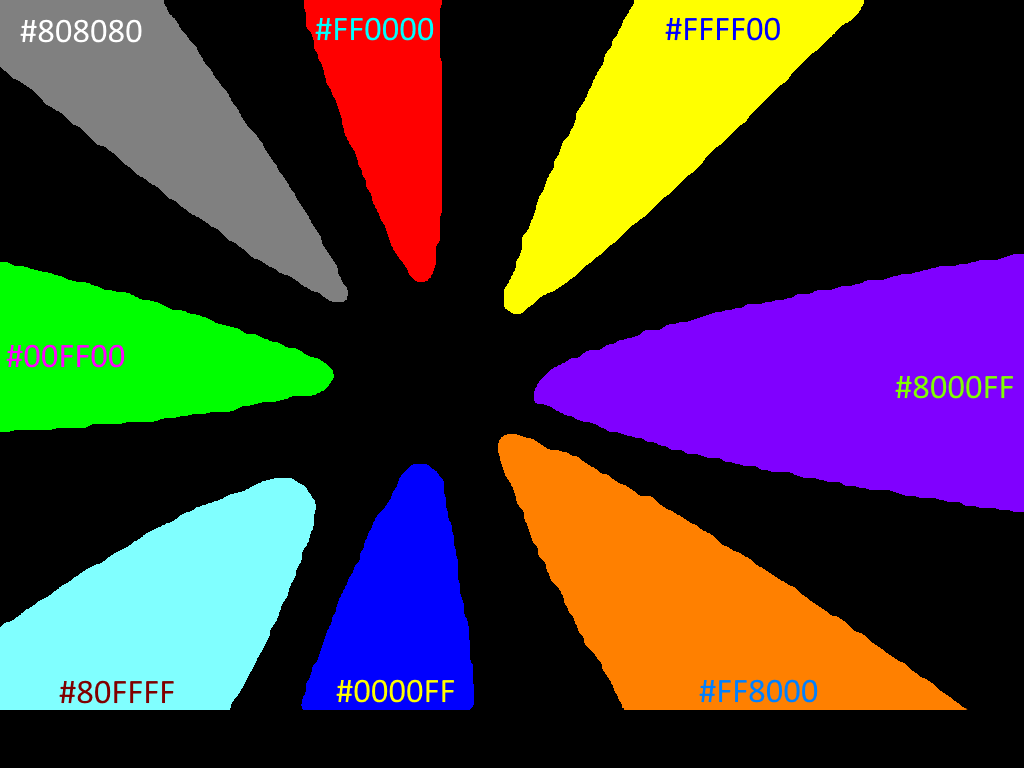
\includegraphics[width=0.45\linewidth]{img/drifttest_stop_017.png}
    }
    \caption{Bild und zugehörige annotierte Maske. Die HEX-Farbwerte sind hier in die Spitzen eingezeichnet.}
    \label{fig:mask}
\end{figure}
Da Photoshop ursprünglich für die Bearbeitung und Verbesserung von Fotografien entwickelt wurde, treten trotz pixelgenauer Auswahl Probleme auf. Denn Photoshop erzeugt keine harten Kanten. Die Farben einiger Grenzpixel vermischen sich leicht.
Dies ist problematisch, da dadurch in den Masken Farben auftreten, die nicht den vordefinierten Farben entsprechen und somit zu Fehlern in der Weiterverarbeitung führen.

Versuche, dieses Problem durch nachträgliche Manipulation von Kontrast, Helligkeit und Sättigung zu beheben, waren nicht erfolgreich. Daher wurde ein Python-Skript zur Nachbearbeitung der annotierten Masken entwickelt.
Genutzt werden dazu die Python Bibliotheken von SciPy \cite{2020SciPy-NMeth}, Pillow \cite{clark2015pillow} und OpenCV \cite{opencv_library}.

Da für die Annotation numerisch gut unterscheidbare Farben gewählt wurden und da ein Pixel – definiert durch das Tupel (r, g, b) – auch als Vektor im dreidimensionalen Raum interpretiert werden kann, lässt sich für jedes Pixel, das von den acht definierten Farben abweicht, die Manhattan-Distanz berechnen und der Wert des Pixels auf den nächstgelegenen Wert setzen.
Auf diese Weise konnten alle Pixelfehler ohne Qualitätsverlust der Annotation beseitigt werden.

\subsection{Konvertierung in das COCO Datenformat}
Mehrere Schritte sind erforderlich, um die erstellten Bilder und annotierten Masken in das COCO-Datenformat zu konvertieren.

Zunächst muss der Datensatz in einen Trainings- und einen Validierungsteil aufgeteilt werden. Zu diesem Zweck werden zwei JSON-Dateien, train.json und val.json, erstellt. In diese Dateien müssen nun alle Klassen, Bilder und Annotationen eingetragen werden.

Um die erstellten Masken in das COCO Format zu übersetzen, müssen zunächst die eingefärbten Spitzen als Polygon dargestellt werden. Dazu werden die Umrisse der eingefärbten Bereiche extrahiert. Zweitens müssen die Bounding-Box-Werte aus den Grenzen des Polygons bestimmt werden. Drittens muss der vorderste Punkt der Spitze bestimmt werden, um den Keypoint zu markieren.
Um diese Aufgaben zu lösen, wird ein Ansatz adaptiert, der von Chris Eijgenstein in seinem Projekt image-to-coco-json-converter genutzt wurde \cite{chriscoco}. Dieser Ansatz verwendet die Python-Bibliotheken shapely \cite{shapely2007}, scikit-image \cite{van2014scikit} und Pillow \cite{clark2015pillow}, um die Konturen der Annotationen aus einem Maskenbild zu extrahieren. Dabei ist zu beachten, dass sich Spitzen überlappen können und somit in 2 Bereiche unterteilt werden. Die Kontur einer Spitzeninstanz wird mit skimage aus dem Bild extrahiert. Shapely stellt die Kontur als Polygon dar und berechnet die Parameter der Bounding Box.
Zur Markierung des Keypoint wird das Binärbild der Kontur mit OpenCV \cite{opencv_library} angezeigt und der Benutzer muss den vordersten Punkt der Spitze entsprechend markieren.
Um ein Maximum an Informationen zu erhalten, werden die acht Spitzen während des gesamten Prozesses als getrennte Klassen behandelt.

Eine Herausforderung besteht darin, eine annotierte Maske mit allen zugehörigen Bildern zu verknüpfen, da sie nach der Konvertierung in das COCO-Format nur über eine ID referenziert wird und nicht über den Dateinamen, wie es bei der Erstellung der Bilder der Fall ist. Zu diesem Zweck werden bereits konvertierte Masken mit Verweis auf ihren Dateinamen zwischengespeichert. Bei nachfolgenden Bildern wird geprüft, ob die zugehörige Maske bereits konvertiert wurde. Falls bereits eine Annotation in COCO-Format vorhanden ist, müssen die Werte \glqq id\grqq{} und \glqq image\_id\grqq{} entsprechend angepasst werden. Dabei ist immer auf die korrekte Nummerierung zu achten, da es sonst zu Konflikten kommen kann.
Es ist notwendig, dass alle anderen Parameter des COCO-Formats ebenfalls korrekt gesetzt sind. Diese sind jedoch trivialer und werden daher hier nicht weiter erläutert.

\subsubsection{Konvertierungsskript}
Zur Automatisierung und Vereinfachung des Konvertierungsprozesses, wird ein spezielles Python-Skript entwickelt. Dieses Skript kann von der Kommandozeile aus aufgerufen werden und ermöglicht es, den gesamten Konvertierungsprozess mit einem einzigen Befehl auszuführen. Es nimmt den Pfad zu dem Ordner als Eingabe und führt dann die Konvertierung durch.
\begin{figure}[h]
\centering
\begin{minipage}{0.4\linewidth}
\dirtree{%
.1 /.
.2 dataset.
.3 images.
.4 image0.tif.
.4 ....
.3 masks.
.4 mask0.png.
.4 ....
.2 dataset-coco.
.3 images.
.4 image0.tif.
.4 ....
.3 annotations.
.4 train.json.
.4 val.json.
}
\end{minipage}
    \caption{Darstellung der Verzeichnisstruktur des Datensatzes vor und nach der Konvertierung. Die Anzahl der erstellten Ordner hängt von der Wahl der Parameter des Konvertierungsskripts ab.}
    \label{fig:folderstruc}
\end{figure}

Jeder erzeugte Datensatz wird in einem separaten Ordner gespeichert, sodass er sofort für Trainingszwecke verwendet werden kann. Die benötigte und erstellte Ordnerstruktur ist in \ref{fig:folderstruc} dargestellt.

Das Besondere an diesem Skript ist seine Flexibilität. Es erlaubt die Spezifikation beliebiger Parameterkombinationen und erzeugt entsprechend die gewünschten Datensätze. Dies ermöglicht die Erstellung maßgeschneiderter Datensätze, die auf spezifische Anforderungen und Anwendungsszenarien zugeschnitten sind. Darüber hinaus ist das Skript einfach zu verstehen und zu warten, was zukünftige Anpassungen und Erweiterungen erleichtert.
Die verfügbaren Skript-Parameter sind in Abbildung \ref{fig:param} aufgelistet.
\begin{figure}
    \centering
\begin{center}
\setlist{noitemsep}
\begin{description}
\item[\texttt{-dataset}] Pfad zum Datensatz (z.B. /home/user/dataset)
\item[\texttt{-split}] Aufteilungsverhältnis Training/Validierung (z.B. 0.8)
\item[\texttt{-coco}] Konvertierung in das COCO-Datenformat
\item[\texttt{-yolo}] Konvertierung in das YOLO-Datenformat
\item[\texttt{-oc}] Verwendung einer einzigen Klasse für alle Spitzen
\item[\texttt{-ib}] Einbeziehung des Hintergrunds für semantische/panoptische Segmentierung
\item[\texttt{-kp}] Einbeziehung der Koordinaten der Schlüsselpunkte
\item[\texttt{-mi}] Verwendung einer Maske für mehrere Bilder
\end{description}
\end{center}
    \caption{Skript-Parameter für die Konvertierung von Datensätzen.}
    \label{fig:param}
\end{figure}
% Ein Beispiel für die Verwendung des Skripts in der Kommandozeile könnte wie folgt aussehen:
% \begin{algorithmic}[htbp]
%     \STATE \text{\$ python convert\_dataset.py -dataset ./50img -split 0.9 -coco -oc -kp}
% \end{algorithmic}
% Dieser Befehl erzeugt aus den Bildern und Masken zwei Datensätze im COCO-Format: einen, in dem alle Spitzen als eine Klasse behandelt werden, und einen, in dem jede Spitze einer eigenen Klasse zugeordnet wird.
% Der Datensatz integriert die Koordinaten der Schlüsselpunkte. Diese müssen für jede Maske zur Laufzeit des Skripts markiert werden. Der Datensatz wird in einen Trainings- und einen Validierungsdatensatz aufgeteilt, wobei 90\% der Daten für das Training und 10\% für die Validierung verwendet werden.
\section{Datensätze}
Um die erforderlichen Skripte zu entwickeln sowie die Entwicklungsumgebung einzurichten und zu testen, wurde eine Reihe von Datensätzen erstellt. Eine tabellarische Übersicht aller Datensätze ist in der Tabelle \ref{tab:datasets} zu finden.
Die Benennung der Datensätze ist intuitiv und natürlich. Der erste Teil des Namens beschreibt die Anzahl der Bilder. Verschiedene Suffixe werden angehängt, um Informationen darüber zu liefern, wie die Masken annotiert sind. Beispielweise steht das Suffix \glqq -oc\grqq{}für \glqq one class\grqq{} (eine Klasse). Die Klassen des Datensatzes sind zusammengefasst. Die Spitzen werden also nicht nach ihrer Richtung unterschieden.

Der Datensatz \glqq 50img\grqq{} enthält 50 Bilder und Masken aus realen Einsatzszenarien. Es diente zur Überprüfung der Annotationsmethode und der Konvertierung in das COCO-Format. Er wurde auch verwendet, um die Entwicklungsumgebung so zu konfigurieren, dass das Training von Mask R-CNN später schnell auf einem großen Datensatz durchgeführt werden kann. 
Der Datensatz \glqq 600img\_1x5\grqq{} enthält 600 Bilder, wobei eine Maske auf fünf Bilder passt, und wurde mit der entwickelten automatischen Bildaufnahmemethode erstellt. Er wird später einen Großteil der Trainingsdaten darstellen.
\glqq 617img\_batch1\grqq{} enthält 100 von insgesamt 617 sorgfältig ausgewählten Bildern aus realen Einsätzen. Sie repräsentieren eine Vielzahl von Szenarien und sollen als Grundlage für eine genaue Darstellung dienen.

Alle Bilder und Masken der oben genannten Datensätze sind in dem Datensatz \glqq 750img\_merged\grqq{} zusammengefasst. Er besteht somit aus 600 Bildern, die durch das Skript erzeugt wurden, und 150 Bildern, die aus realen Einsätzen stammen. Nach einer genaueren Analyse des Datensatzes stellte sich heraus, dass Spitzen aus verschiedenen Richtungen unterschiedlich häufig in den Bildern vertreten sind. Dies wird auf die 150 Bilder aus realen Einsätzen zurückgeführt. Dargestellt ist die Verteilung in Abbildung \ref{fig:instpclass}. Es zeigt sich, dass insbesondere die Spitzen fünf (Süd) und sechs (Süd-West) seltener im Einsatz sind. Dennoch wird der Datensatz für das Training von Mask R-CNN verwendet und in der Evaluierung wird untersucht, inwieweit sich dieses Ungleichgewicht auf die Leistungsfähigkeit des Modells auswirkt.
\begin{table}[h]
\begin{adjustbox}{width=\columnwidth,center}
\begin{tabular}{llllll}
\toprule
\textbf{Name} & \textbf{Bildanzahl} & \textbf{Augmentation} & \textbf{Klassen} & \textbf{Entwicklung} & \textbf{Training} \\
\midrule
50img         & 50                  & Nein                     & 8                 & Ja                    & Nein              \\
50img-oc      & 50                  & Nein                   & 1                 & Ja                    & Nein              \\
600img\_1x5        & 600                 & Ja                     & 8                 & Ja                    & Nein              \\
617img\_batch1     & 100                 & Nein                   & 8                 & Nein                  & Nein              \\
750img\_merged        & 750                 & Teils                     & 8                 & Nein                  & Ja                \\
750img\_merged-oc     & 750                 & Teils                     & 1                 & Nein                  & Ja                \\
\bottomrule
\end{tabular}
\end{adjustbox}
\caption{Zusammenfassung der Datensätze. Alle Datensätze haben ein Train-Val-Verhältnis von 0.9}
\label{tab:datasets}
\end{table}

% \begin{figure}[htbp]
%     \centering
%     \begin{tikzpicture}
%         \begin{axis}[
%             ybar,
%             bar width=0.5cm,
%             width=12cm,
%             height=8cm,
%             xlabel={Tip},
%             ylabel={Anzahl},
%             symbolic x coords={tip1, tip2, tip3, tip4, tip5, tip6, tip7, tip8},
%             enlargelimits=0.15,
%             legend style={at={(0.5,-0.15)},
%                 anchor=north,legend columns=-1},
%             xtick=data,
%             nodes near coords,
%             nodes near coords align={vertical},
%             ymin=0
%         ]
%         \addplot coordinates {(tip1, 35) (tip2, 14) (tip3, 32) (tip4, 19) (tip5, 34) (tip6, 12) (tip7, 32) (tip8, 15)};
%         \addplot coordinates {(tip1, 528) (tip2, 556) (tip3, 482) (tip4, 406) (tip5, 293) (tip6, 293) (tip7, 589) (tip8, 503)};
%         \legend{50img, 750img\_merged}
%         \end{axis}
%     \end{tikzpicture}
%     \caption{Verteilung der Klassen im Entwicklungs- und Trainingsdatensatz. 50img enthält 193 Instanzen. 750img\_merged enthält 3650 Instanzen. Es fällt auf, dass insbesondere die Klassen tip5 und tip6 in den Daten unterrepräsentiert sind.}
%     \label{fig:my_bar_chart}
% \end{figure}
\begin{figure}[h]
    \centering
    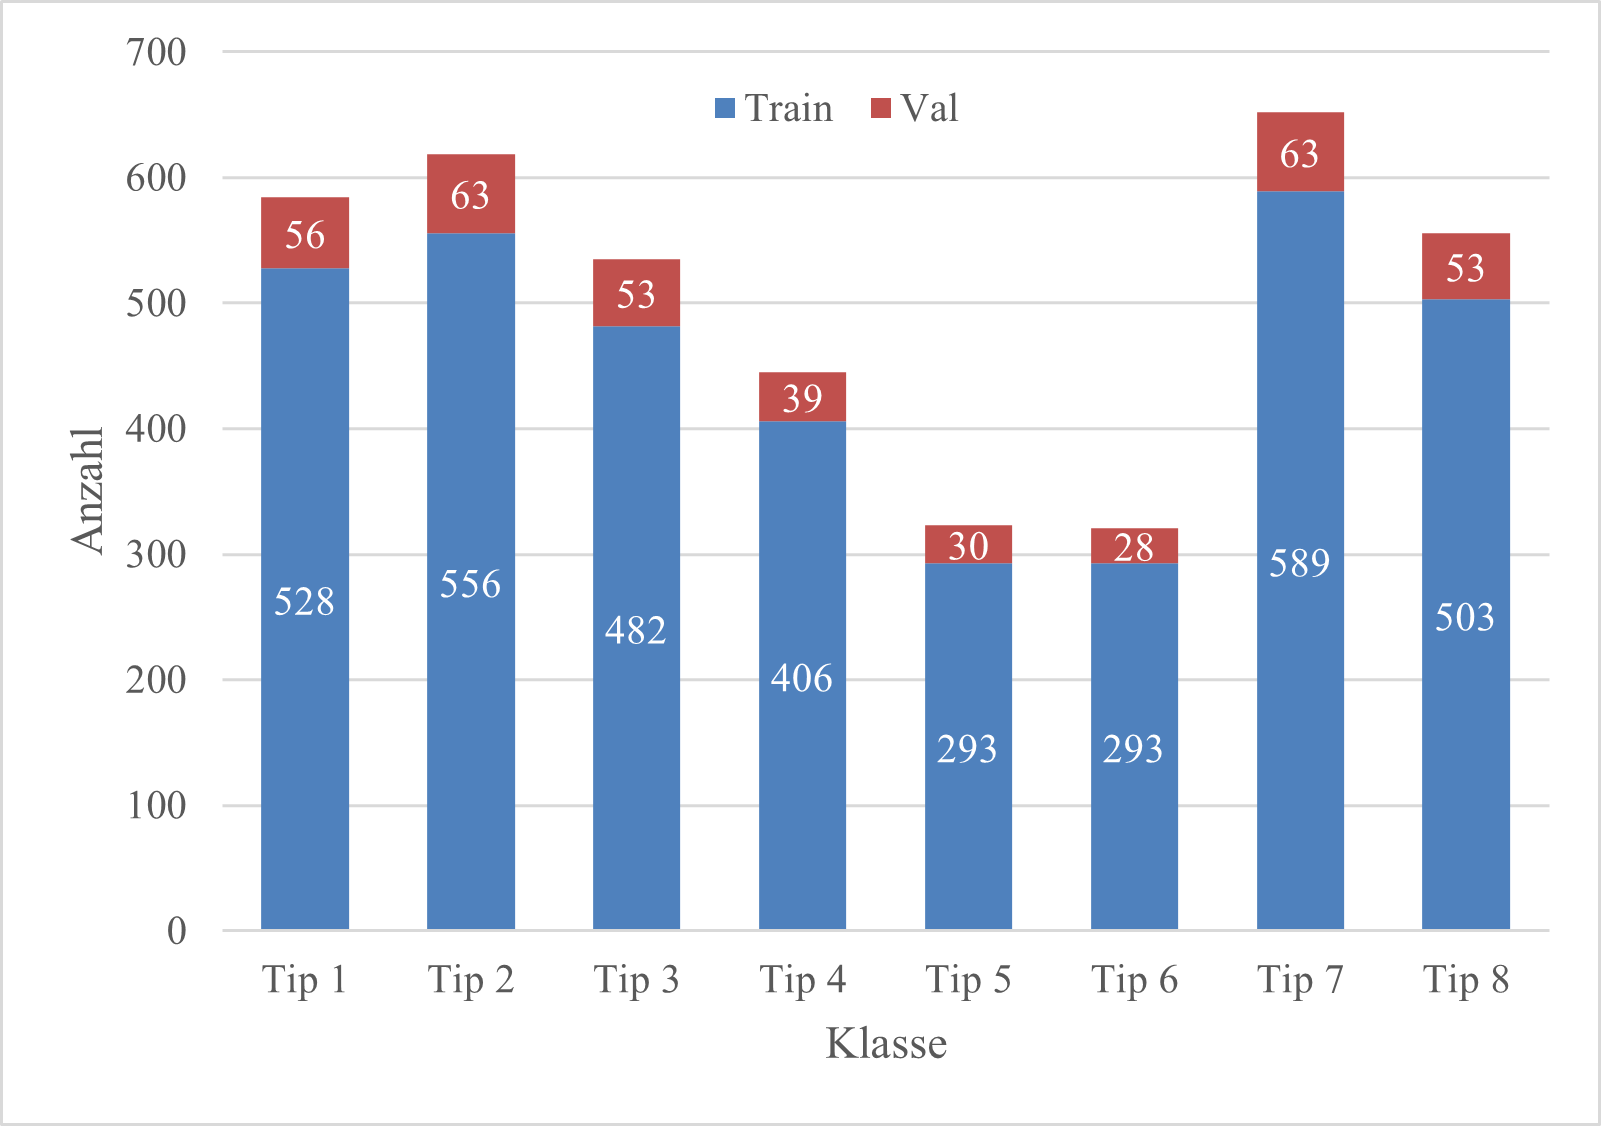
\includegraphics[trim={0.2cm 0.2cm 0.2cm 0.2cm}, clip]{img/eval/inst_per_class.png}
    \caption{Anzahl der Instanzen jeder Spitzenklasse von \glqq 750img\_merged\grqq{}. Dies ermöglicht einen Vergleich zwischen den Klassenverteilungen in den Trainings- und Validierungsdaten.}
    \label{fig:instpclass}
\end{figure}

\clearpage
\section{Implementierung und Training der Modelle}
\subsection{Entwicklungsumgebung}
Für diese Entwicklung wird ein System mit Ubuntu in der Version 22.04 verwendet. Die effiziente Nutzung der zugrunde liegenden Grafikkarte vom Typ \glqq Nvidia GTX 1080\grqq{} wird durch die Installation von CUDA 11.8 erreicht, einer von Nvidia entwickelten parallelen Berechnungsplattform und Anwendungsprogrammierschnittstelle (API). CUDA ermöglicht es Entwicklern, Software zu schreiben, die die Hardwarebeschleunigung für rechenintensive Anwendungen nutzt, insbesondere in den Bereichen maschinelles Lernen und Datenverarbeitung \cite{cuda}.

Für die Entwicklung der Netze wird PyTorch in der Version 2.0.1 zusammen mit torchvision-0.15.1 installiert. PyTorch ist ein Open-Source-Maschinelearning-Framework, das die schnelle Entwicklung von Deep Learning-Algorithmen ermöglicht. Es bietet sowohl flexible als auch effiziente Implementierungen von verschiedenen Arten von neuronalen Netzen und anderen maschinellen Lern-Algorithmen \cite{NEURIPS2019_9015}. Die entsprechenden Versionen wurden vorab für CUDA 11.8 kompiliert, um das Training auf der Grafikkarte zu ermöglichen und damit zu beschleunigen.

Für das Training der Netze wird Detectron2 verwendet. Da für diese spezielle Systemkonfiguration keine vorkompilierte Version von Detectron2 verfügbar ist, wird sie aus dem Quellcode erstellt.

Die oben beschriebene Entwicklungsumgebung wird hauptsächlich für die Vor- und Nachverarbeitung der Daten sowie für die Implementierung und das Debugging des Mask R-CNN Modells verwendet. Da diese Umgebung jedoch nicht die erforderliche Rechenleistung für ein schnelles und effizientes Training des Modells bietet, wird das Training selbst in einer Cloud-basierten Umgebung, konkret auf Google Colab, durchgeführt.

Google Colab ist eine Cloud-Service-Plattform, die GPU-Ressourcen für maschinelles Lernen und datenwissenschaftliche Forschung zur Verfügung stellt \cite{google-colab}.
Für das Training wird eine Instanz mit einer Nvidia V100 Grafikkarte ausgewählt. Die Nvidia V100 ist eine Hochleistungs-GPU, die speziell für maschinelles Lernen und rechenintensive Anwendungen entwickelt wurde. Sie bietet eine erhebliche Beschleunigung im Vergleich zu Consumer-Grafikkarten und ist mit 16 Gigabyte Grafikspeicher ideal für das Training von Deep Learning Modellen geeignet.
In dieser Google Colab Umgebung ist es notwendig, Detectron2 zu installieren. Durch den Einsatz von Google Colab kann trotz der Hardwarebeschränkungen der lokalen Entwicklungsumgebung ein effizientes Training des Modells erreicht werden.
\subsection{Implementierung von Mask R-CNN}
Der sogenannte \glqq Model Zoo\grqq{} von Detectron2, eine Sammlung von vorgefertigten Modellen und Konfigurationen für verschiedene Algorithmen und deren Varianten enthält auch verschiedene Implementierungen von Mask R-CNN und Keypoint R-CNN, die als Ausgangspunkt für das in dieser Arbeit verwendete Modell dienten.

Mask R-CNN wurde aufgrund seiner Modularität ausgewählt. Es kann schnell angepasst werden, um Objektdetektion, Segmentierung und Keypoint-Erkennung durchzuführen, andere Modellarchitekturen bieten diese Flexibilität nicht.

Von besonderem Interesse sind die verschiedenen Backbone-Architekturen, die im Model Zoo von Detectron2 zur Verfügung stehen. Es werden die Backbones R50-FPN, R50-DC5, R101-FPN und R101-DC5 verwendet.
Eine detaillierte Erläuterung der Backbones findet sich in Kapitel \ref{sec:backbone}.

% , hier jedoch eine kurze Zusammenfassung.
% ResNet-50 (R50) und ResNet-101 (R101) sind Varianten des ResNet-Modells, die eine effiziente Lösung für das Problem des verschwindenden Gradienten in tiefen neuronalen Netzen bieten. FPN steht für Feature Pyramid Network, eine Netzarchitektur, die Informationen aus mehreren Extraktionsebenen verwendet, um die Genauigkeit der Objekterkennung zu verbessern. DC5 bezeichnet eine Konfiguration, bei der alle 3x3-Convolutions in der C5-Stufe von ResNet durch 3x3-Dilated-Convolutions ersetzt werden.

\begin{figure}[h]
    \centering
    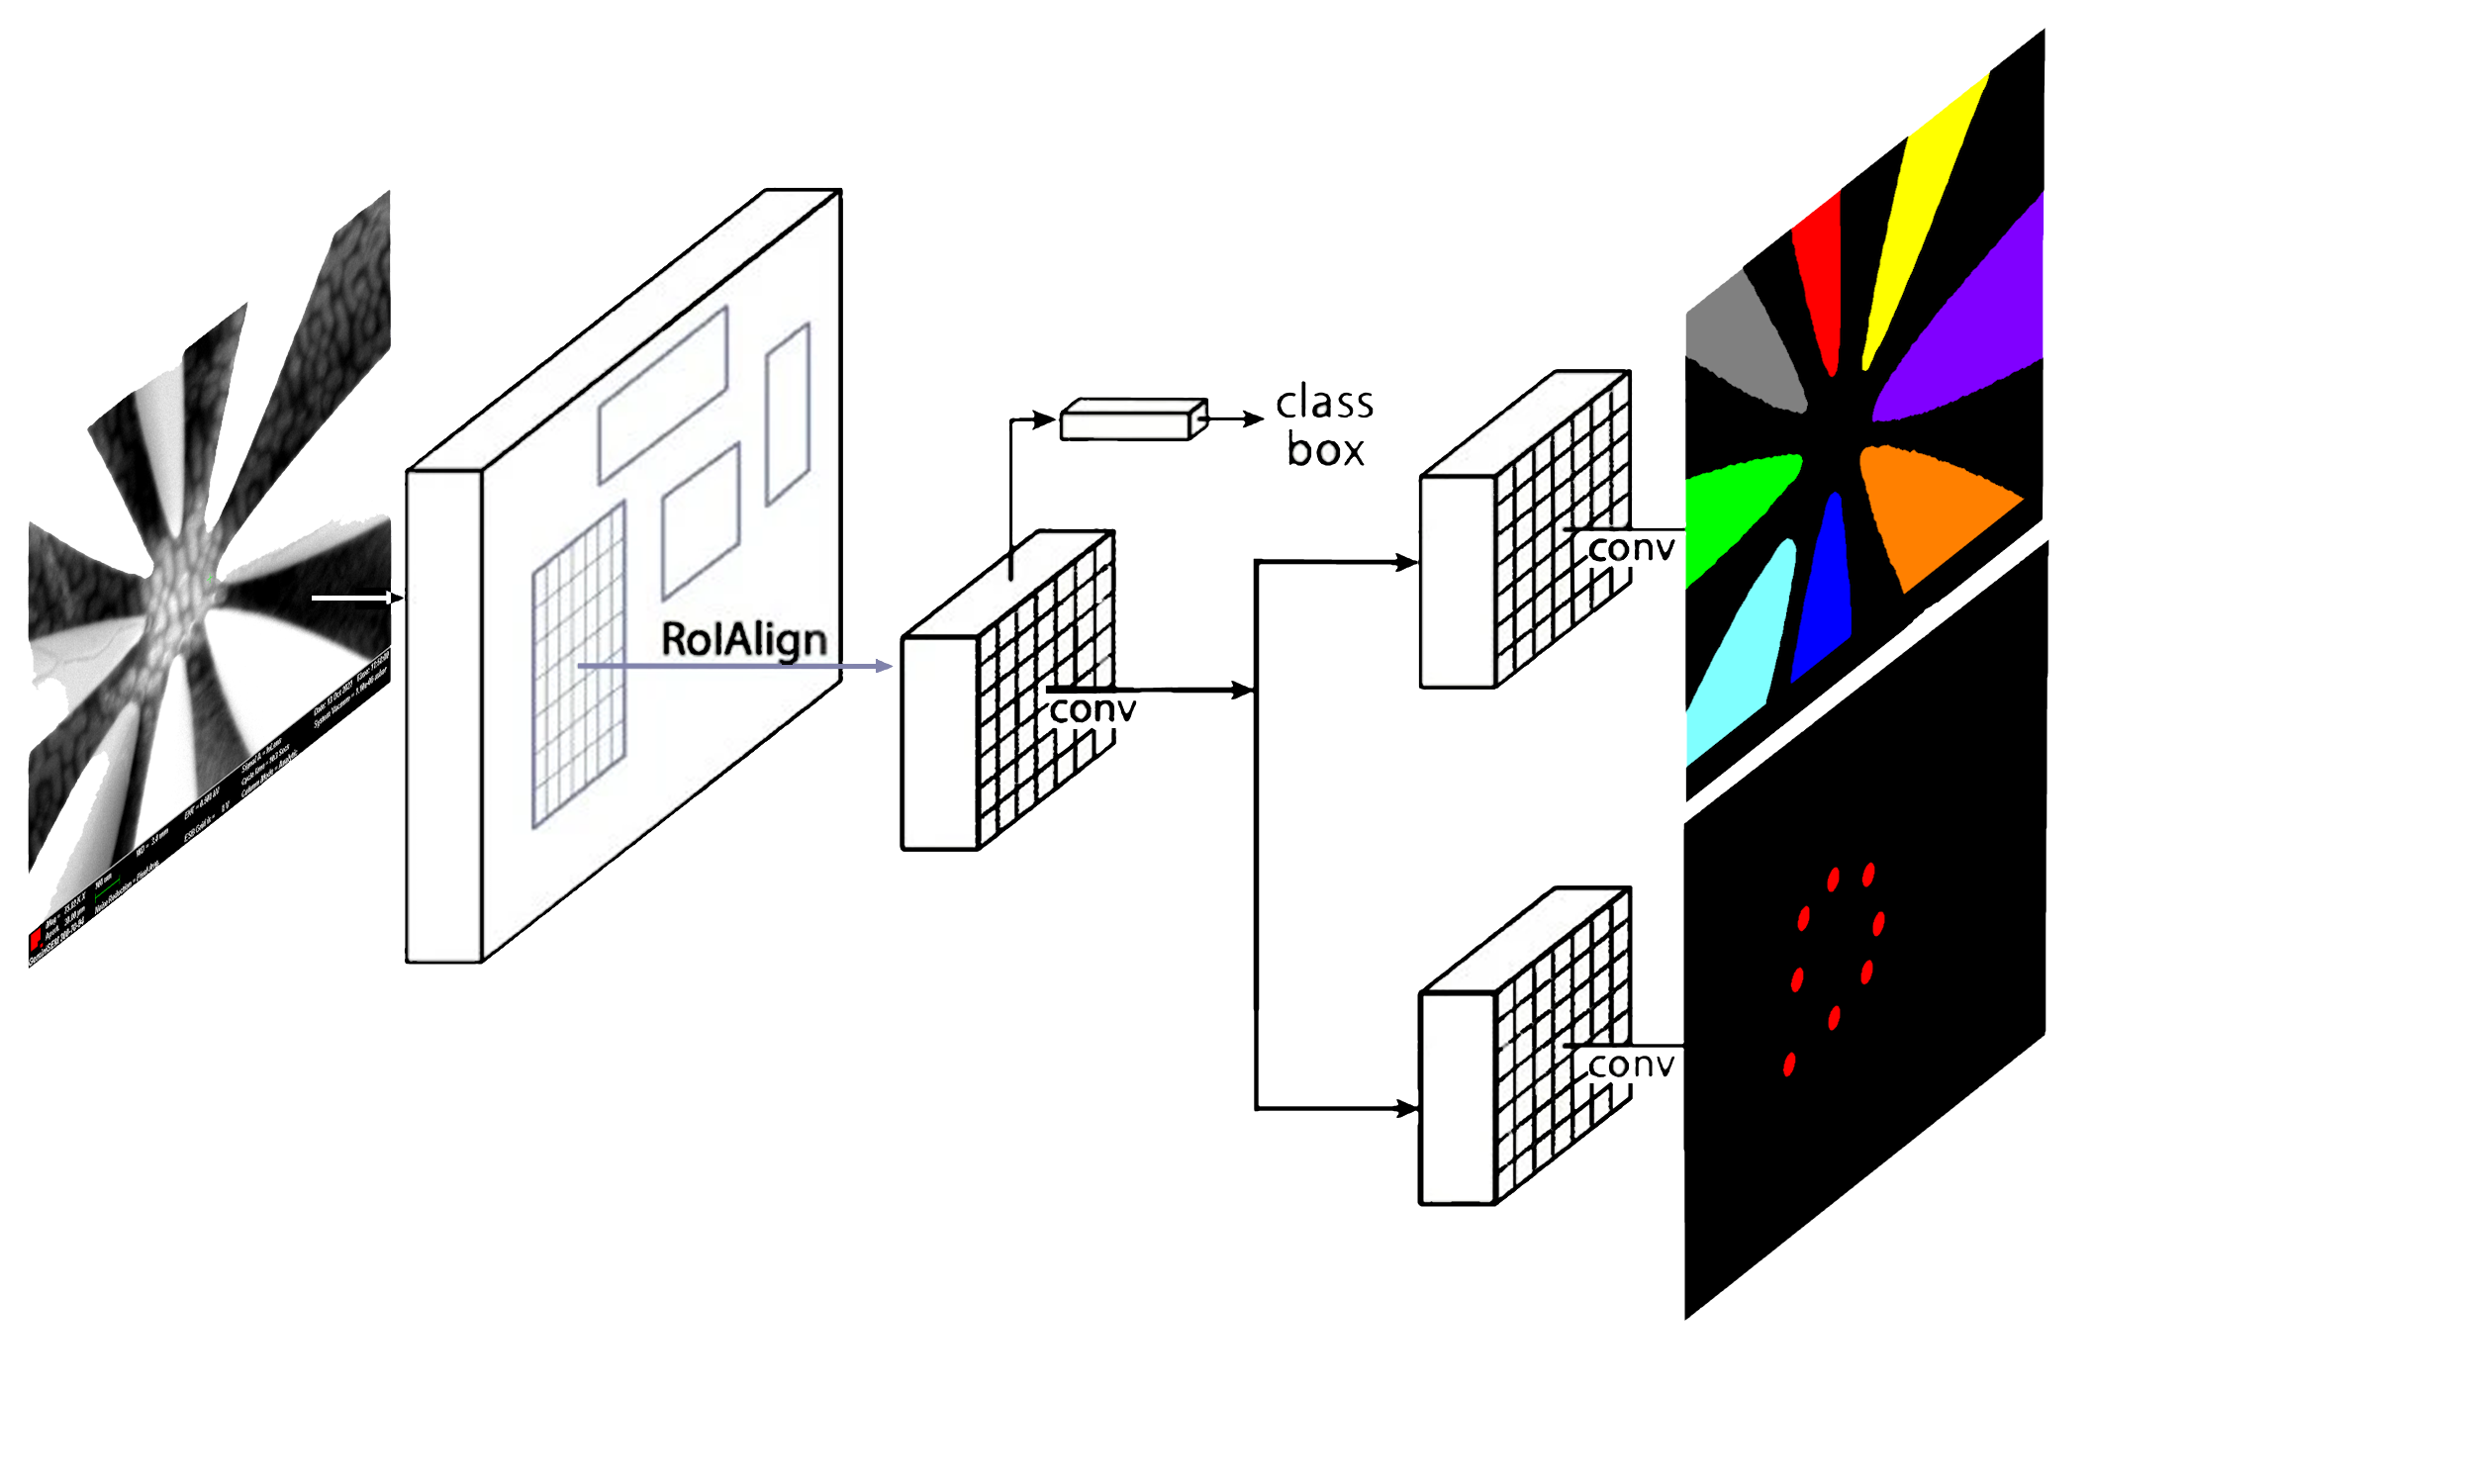
\includegraphics[width=0.8\linewidth, clip, trim={0 4cm 10cm 0.5cm}]{img/model_arch.png}
    \captionsource{Die verwendete Mask R-CNN Architektur, der Keypoint-Zweig wird angefügt. Die Keypoints werden als eine One-Hot Maske ausgegeben.}{Modifiziert übernommen von He \textit{et al.} \cite{He_2017_ICCV}}
    \label{fig:modelarch}
\end{figure}
Da das Modell sowohl Schlüsselpunkte als auch Segmentierungsmasken ausgeben soll, werden die entsprechenden Konfigurationen von Mask R-CNN und Keypoint R-CNN zusammengefasst, die Architektur ist in Abbildung \ref{fig:modelarch} dargestellt. Auf diese Weise können die Vorteile beider Modelltypen genutzt werden und das Modell erzeugt beide Ausgaben gleichzeitig.

Die Konfigurationen werden entsprechend den spezifischen Anforderungen dieser Arbeit angepasst, wobei die Details der Anpassungen im Abschnitt \ref{sec:hyperp} über die Einstellung der Hyperparameter näher beschrieben werden. Mit diesen Einstellungen konnte ein maßgeschneidertes Mask R-CNN Modell entwickelt werden, das speziell für die Aufgabe der Lokalisierung von Messspitzen im REM geeignet ist.
\subsection{Verwendung und Anpassung der vortrainierten Gewichte}
%Durch die Verwendung vortrainierter Gewichte kann das Modell effizienter trainiert werden. Dies bedeutet, dass das Modell auf den bereits gelernten Eigenschaften der vortrainierten Gewichte aufbaut, was den Trainingsprozess beschleunigt und eine bessere Leistung des Modells ermöglicht, als wenn das Modell von Grund auf neu trainiert würde.
Für diese Arbeit werden verschiedene vortrainierte Modelle aus dem Detectron2 Model Zoo verwendet, aufgelistet sind diese in Tabelle \ref{tab:modelle}.
Diese Modelle wurden ursprünglich auf dem COCO \glqq train2017\grqq{} Datensatz trainiert, einem großen und vielfältigen Datensatz zur Objekterkennung, Segmentierung und Keypoint-Erkennung \cite{coco}.

Da das Modell zur Spitzenerkennung beide Fähigkeiten – Masken- und Keypoint-Vorhersage – beherrschen soll, werden die vortrainierten Gewichte des Keypoint-Zweiges aus den Keypoint R-CNN-Modellen extrahiert und mit den Parametern des entsprechenden Mask R-CNN-Modells mithilfe eines Python-Skripts kombiniert. Dies ermöglicht die Erstellung eines vortrainierten Modells, das sowohl die bereits erlernten Fähigkeiten zur Maskengenerierung als auch zur Keypoint-Erkennung besitzt.

\begin{table}[h]
\centering
\begin{tabular}{lll}
\toprule
\textbf{Name} & \textbf{Backbone} & \textbf{LR Schedule} \\
\midrule
Mask R-CNN & R50-DC5 & 3x \\
Mask R-CNN & R50-FPN & 3x \\
Keypoint R-CNN & R50-FPN & 3x \\
Mask R-CNN & R101-FPN & 3x \\
Mask R-CNN & R101-DC5 & 3x \\
Keypoint R-CNN & R101-FPN & 3x \\
\bottomrule
\end{tabular}
\caption{Genutzte vortrainierte Modelle aus dem Detectron2 Model Zoo.}
\label{tab:modelle}
\end{table}
Es ist jedoch anzumerken, dass für die DC5 Varianten der Backbones keine vortrainierten Gewichte für den Keypoint-Zweig zur Verfügung stehen. In diesem Fall wird das Modell nur mit den verfügbaren Mask R-CNN Gewichten trainiert.

Um den vollen Nutzen aus den vortrainierten Gewichten zu ziehen, wird ein spezielles Trainingsschema verwendet. In einer ersten Phase wird das Backbone des Modells \glqq eingefroren\grqq{}, das heißt, es werden keine Gradienten berechnet und die Gewichte werden nicht aktualisiert. Dadurch kann der Maskenkopf des Modells lernen, die Positionen und Konturen der Spitzen auf Grundlage der bereits gelernten Merkmale des Backbone zu rekonstruieren.
In der zweiten Phase des Trainingsprozesses wird das gesamte Modell einschließlich des Backbones auf dem spezifischen Datensatz trainiert. Dieser Schritt stellt sicher, dass das Modell genau an die spezifische Aufgabe angepasst ist. Zur Unterstützung dieses zweiphasigen Trainingsprozesses wird eine speziell angepasste Lernrate verwendet, die den Fortschritt des Modells in beiden Phasen effektiv steuert. Die entwickelte Lernrate ist in Abbildung \ref{fig:lr} zu sehen.
\subsection{Wahl der Hyperparameter}
\label{sec:hyperp}
In Detectron2 wird für das Training auf acht GPUs eine Lernrate von 0,02 verwendet. Die lineare Skalierungsregel von Goyal \textit{et al.} \cite{1706.02677} besagt, dass die Lernrate proportional zur Anzahl der GPUs angepasst werden sollte. Daher wird die anfängliche Lernrate für das Training auf einer einzelnen GPU auf 0,002 reduziert.

Für den Optimierer wird ein Momentum-Wert von 0,9 festgelegt. Dies hilft, den Trainingsprozess in die richtige Richtung zu beschleunigen. Eine Gewichtsabnahme von 0,0001 wird verwendet, und reguliert  die Überanpassung.
16 Bilder pro Batch sind die optimale Anzahl, um die Leistung der Nvidia V100 GPU voll auszunutzen, ohne sie zu überlasten. Dies trägt zu einer effizienten Nutzung der Hardware-Ressourcen bei, ohne die Qualität des Trainings zu beeinträchtigen.

\begin{figure}[h]
    \centering
    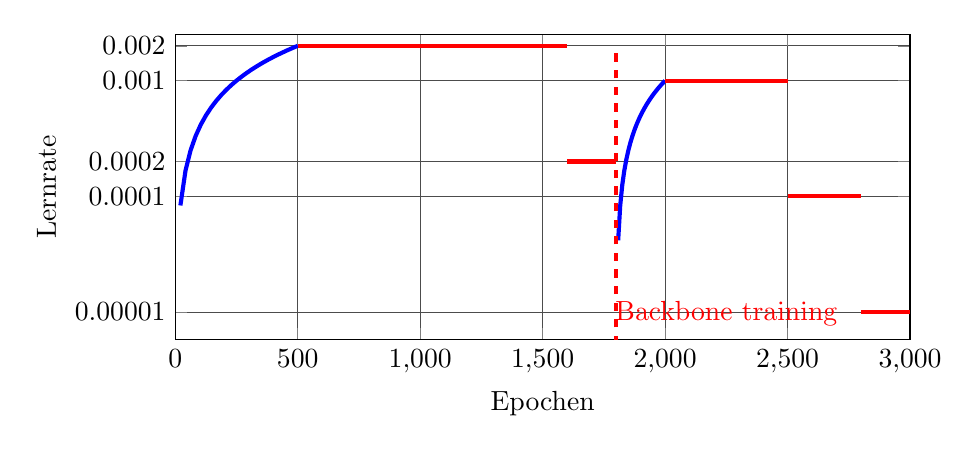
\begin{tikzpicture}
        \begin{axis}[
            xlabel=Epochen,
            ylabel=Lernrate,
            xmin=0, xmax=3000,
            ymin=0, ymax=0.0025,
            height=0.45\textwidth,
            width=0.9\textwidth,
            ymode=log, % Set the y-axis to log scale
            xtick={0,500,1000,1500,2000,2500,3000},
            ytick={0.00001, 0.0001, 0.0002, 0.001, 0.002},
            yticklabels={0.00001, 0.0001, 0.0002, 0.001, 0.002}, % Set the tick labels
            ytickten={-5, -4, -3, -2, -1}, % Specify the power of 10 for the ticks
            grid=both,
            grid style={line width=.3pt, draw=black!70},
        ]
            % First linear segment
            \addplot[domain=0:500, blue, line width=1.5pt] {0.002*x/500};
            
            % Constant segment
            \addplot[domain=500:1600, red, line width=1.5pt] {0.002};
            
            % Second linear segment
            \addplot[domain=1600:1800, red, line width=1.5pt] {0.0002};
            
            % Third linear segment
            \addplot[domain=1800:2000, blue, line width=1.5pt] {0.001*(x-1800)/200};
            
            % Constant segment
            \addplot[domain=2000:2500, red, line width=1.5pt] {0.001};
            
            % Fourth linear segment
            \addplot[domain=2500:2800, red, line width=1.5pt] {0.0001};
            
            % Fifth linear segment
            \addplot[domain=2800:3000, red, line width=1.5pt] {0.00001};

            \draw [red, dashed, line width=1.5pt] (axis cs:1800, 0.0000001) -- (axis cs:1800, 0.002);
            \node[anchor=north, red] at (axis cs:2250, 0.000015) {Backbone training};
        \end{axis}
    \end{tikzpicture}
    \caption{Der Verlauf der Lernrate über die Epochen, logarithmisch dargestellt. Lernrate der Aufwärmepochen in Blau, konstante Lernrate in Rot.}
    \label{fig:lr}
\end{figure}
Die Modelle werden für 3000 Epochen trainiert. Während der Entwicklung und Erprobung hat sich diese Zahl als optimal für ein ausgewogenes Verhältnis zwischen Modellleistung und Trainingszeit erwiesen.
Die ersten 500 Epochen des Trainings dienen als Aufwärmphase. In dieser Phase wird die Lernrate schrittweise linear auf die eingestellte Lernrate erhöht. Liu \textit{et al.} haben gezeigt, dass dieser Vorgang dazu beitragen kann, das Modell besser auf das Training vorzubereiten und Instabilitäten zu Beginn des Trainings zu vermeiden \cite{1908.03265}.

In den ersten 1800 Epochen werden die Masken und der Keypoint-Kopf trainiert, während das Backbone-Modell eingefroren bleibt. Die folgenden 1200 Epochen dienen der Feinabstimmung des gesamten Modells, einschließlich des Backbones. Diese zweite Trainingsphase beginnt wieder mit einer Aufwärmphase von 200 Epochen.

Die Lernrate wird während des Trainings in festgelegten Schritten abgestuft und reduziert, einerseits um die Modellkonvergenz zu fördern und andererseits ein Überspringen des globalen Minimums zu verhindern. Diese Anpassung ermöglicht eine anfänglich breitere Exploration des Lösungsraums und eine anschließende feinere Suche, wenn sich das Modell der optimalen Lösung nähert. Die entwickelte Strategie in Abbildung \ref{fig:lr} dargestellt.
\subsection{Erweiterung der Modelle: Richtungsvorhersage}
In einem weiteren Schritt werden die beiden Modellvarianten, die die beste Leistung bei der Erkennung von Spitzen aus allen Richtungen zeigen, erweitert. Dazu werden sie modifiziert und auf dem Datensatz \glqq 750\_merged\grqq{} trainiert. Die Spitzen werden nun nicht nur allgemein, sondern speziell nach ihrer Richtung unterschieden. Dahinter steht die Annahme, dass ein Modell, das in der Lage ist, Spitzen aus allen Richtungen zu erkennen, auch in der Lage sein könnte, diese Spitzen anhand ihrer spezifischen Position zu unterscheiden. Dies würde eine wesentliche Verbesserung für die automatisierte Steuerung darstellen, da eine nachträgliche Zuordnung der Segmentierung und der Schlüsselpunkte zur richtigen Spitze nicht mehr erforderlich wäre.

Es ist jedoch zu berücksichtigen, dass durch die spezifische Klassifizierung der Spitzen für jede Klasse insgesamt weniger Trainingsbilder zur Verfügung stehen. In einem ausgewogenen Datensatz führt dies zu einer Reduktion der Datenmenge auf ein Achtel pro Klasse. Dies stellt eine zusätzliche Herausforderung dar, da das Modell nun feinere Unterscheidungen treffen muss, während die Anzahl der Trainingsbeispiele pro Klasse reduziert wird.

Trotz der feineren Unterscheidung der Spitzen könnte die Aufgabe aus einer anderen Perspektive einfacher sein.
Da die Spitzen annähernd die gleichen Eigenschaften haben und sich hauptsächlich in ihrer Ausrichtung unterscheiden, muss jede der acht Masken Zweige des Modells nur eine der acht möglichen Darstellungen lernen. Da die auf eine Klasse trainierten Modelle bereits die Merkmale der Spitzen gelernt haben, werden die vortrainierten Backbones als Basis für die erweiterten Modelle verwendet. Die Masken-Zweige von Mask R-CNN werden von Grund auf neu trainiert.

Eine sorgfältige Bewertung der Leistung der Modelle ist entscheidend, um das Verhalten der Vorhersagen zu bestimmen, wenn das Modell auf diese Weise trainiert wird.